% !TEX TS-program = xelatex
% Command for running this example (needs latexmkrc file):
%    latexmk -bibtex -pdf main.tex

%	نمونه پایان‌نامه آماده شده با استفاده از کلاس tehran-thesis، نگارش 1
%	سینا ممکن، دانشگاه تهران 
%	https://github.com/sinamomken/tehran-thesis
%	گروه پارسی‌لاتک
%	http://www.parsilatex.com
%	این نسخه، بر اساس نسخه‌ 0.1 از کلاس IUST-Thesis آقای محمود امین‌طوسی آماده شده است.
%        http://profsite.sttu.ac.ir/mamintoosi

%----------------------------------------------------------------------------------------------
% اگر قصد نوشتن پروژه کارشناسی را دارید، در خط زیر به جای msc، کلمه bsc و اگر قصد نوشتن رساله دکترا را دارید، کلمه phd را قرار دهید. کلیه تنظیمات لازم، به طور خودکار، اعمال می‌شود.

% اگر مایلید پایان‌نامه شما دورو باشد به جای oneside در خط زیر از twoside استفاده کنید.

% برای حاشیه‌نویسی و کم کردن صفحات ابتدایی، گزینه draft را وارد و برای نسخه نهایی آن را حذف کنید.

% برای استفاده از قلم‌های سری IR Series گزینه irfonts را وارد و برای استفاده از قلم‌های X Series 2 آن را حذف کنید.

\documentclass[
twoside
% ,openany
,bsc
,irfonts
% ,draft
]{./tex/tehran-thesis}

\newcommand{\mc}[1]{\mathcal{#1}}



% فایل commands.tex را مطالعه کنید؛ چون دستورات مربوط به فراخوانی بسته‌ها، فونت و دستورات خاص در این فایل قرار دارد.
% در این فایل، دستورها و تنظیمات مورد نیاز، آورده شده است.
%-------------------------------------------------------------------------------------------------------------------
% دستوراتی که پوشه پیش‌فرض زیرفایل‌های tex را مشخص می‌کند.
%\makeatletter
%\def\input@path{{./tex/}}
%\makeatother
% در ورژن جدید زی‌پرشین برای تایپ متن‌های ریاضی، این سه بسته، حتماً باید فراخوانی شود
\usepackage{amsthm,amssymb,amsmath}
% بسته‌ای برای تنطیم حاشیه‌های بالا، پایین، چپ و راست صفحه
\usepackage[a4paper, top=40mm, bottom=40mm, outer=25mm, inner=35mm]{geometry}
% بسته‌‌ای برای ظاهر شدن شکل‌ها و تعیین آدرس تصاویر
\usepackage[final]{graphicx}
\usepackage{booktabs}
\graphicspath{{./img/}}
% بسته‌های مورد نیاز برای نوشتن کدها، رنگ‌آمیزی آنها و تعیین پوشهٔ کدها
\usepackage[final]{listings}
\usepackage[usenames,dvipsnames,svgnames,table]{xcolor}
\lstset{inputpath=./code/}
% بسته‌ای برای رسم کادر
\usepackage{framed} 
% بسته‌‌ای برای چاپ شدن خودکار تعداد صفحات در صفحه «معرفی پایان‌نامه»
\usepackage{lastpage}
% بسته‌ٔ لازم برای: ۱. تغییر شماره‌گذاری صفحات پیوست. ۲. تصحیح باگ آدرس وب حاوی '%' در مراجع
\usepackage{etoolbox}

%%%%%%%%%%%%%%%%%%%%%%%%%%%%%%%%%%%%
%%% دستورات وابسته به استیل مراجع:
%% اگر از استیل‌های natbib (plainnat-fa، asa-fa، chicago-fa) استفاده می‌کنید، خط زیر را فعال و بعدی‌اش را غیرفعال کنید.
%\usepackage{natbib}
%\newcommand{\citelatin}[1]{\cite{#1}\LTRfootnote{\citeauthor*{#1}}}
%\newcommand{\citeplatin}[1]{\citep{#1}\LTRfootnote{\citeauthor*{#1}}}
%% اگر از سایر استیل‌ها استفاده می‌کنید، خط بالا را غیرفعال و خط‌های زیر را فعال کنید.
\let\citep\cite
\let\citelatin\cite
\let\citeplatin\cite
%%%%%%%%%%%%
% بررسی حالت پیش نویس
\usepackage{ifdraft}
\ifdraft
{%
	% بسته‌ٔ ایجاد لینک‌های رنگی با امکان جهش
	\usepackage[unicode=true,pagebackref=true,
colorlinks,linkcolor=blue,citecolor=blue,final]{hyperref}
	%\usepackage{todonotes}
	\usepackage[firstpage]{draftwatermark}
	\SetWatermarkText{\ \ \ پیش‌نویس}
	\SetWatermarkScale{1.2}
}
{ 
	\usepackage[pagebackref=false]{hyperref}
	%\usepackage[disable]{todonotes} % final without TODOs
}

\usepackage[obeyDraft]{todonotes}
\setlength{\marginparwidth}{2cm}

\usepackage{tikz}
\usepackage{tikzit}
\usepackage{pgfplots}
%\usepackage{subcaption}
% \usepackage{hyperref}

\usepackage{anyfontsize}
% TiKZ style file generated by TikZiT. You may edit this file manually,
% but some things (e.g. comments) may be overwritten. To be readable in
% TikZiT, the only non-comment lines must be of the form:
% \tikzstyle{NAME}=[PROPERTY LIST]

% Node styles
\tikzstyle{node}=[fill={rgb,255: red,165; green,162; blue,255}, draw={rgb,255: red,51; green,42; blue,179}, shape=circle, minimum size=10]
\tikzstyle{empty_node}=[draw={rgb,255: red,51; green,42; blue,179}, shape=circle]
\tikzstyle{Rec}=[draw=black, shape=rectangle, minimum width=3cm, minimum height=3.5cm]
\tikzstyle{X_wrapper}=[draw=black, shape=rectangle, minimum width=3cm, minimum height=3cm]
\tikzstyle{red_node}=[fill={rgb,255: red,255; green,185; blue,186}, draw={rgb,255: red,143; green,21; blue,38}, shape=circle]
\tikzstyle{layer_1_wrapper}=[draw=black, shape=rectangle, minimum width=4cm, minimum height=16.5cm, line width=3pt, rounded corners=0.4cm]
\tikzstyle{second_laeyr_wrapper}=[draw={rgb,255: red,51; green,11; blue,121}, shape=rectangle, minimum width=4cm, minimum height=28cm, fill={rgb,255: red,158; green,160; blue,255}, opacity=0.2, rounded corners=0.4cm]
\tikzstyle{EncoderWrapper}=[draw=black, shape=rectangle, minimum width=42cm, line width=5pt, minimum height=36cm, rounded corners=0.4cm]
\tikzstyle{description}=[inner sep=0mm, font={\fontsize{55}{50}\selectfont}]
\tikzstyle{description_layers}=[inner sep=0mm, font={\fontsize{45}{43}\selectfont}]
\tikzstyle{InputsWrapper}=[draw=black, shape=rectangle, minimum width=6.5cm, minimum height=8.5cm, rounded corners=0.2cm, line width=5pt]
\tikzstyle{MiniInputsWrapper}=[draw=black, shape=rectangle, minimum width=7cm, minimum height=8.5cm, rounded corners=0.2cm, line width=5pt]
\tikzstyle{Zprim}=[draw=black, shape=rectangle, minimum width=8.5cm, minimum height=6cm, rounded corners=0.2cm, line width=5pt]
\tikzstyle{Pz}=[draw=black, shape=rectangle, minimum width=8.5cm, minimum height=9cm, rounded corners=0.2cm, line width=5pt]
\tikzstyle{little_node}=[fill={rgb,255: red,165; green,162; blue,255}, draw={rgb,255: red,51; green,42; blue,179}, shape=circle, minimum size=0.01cm]
\tikzstyle{OutputsWrapper}=[draw=black, shape=rectangle, minimum width=4.5cm, minimum height=7cm, rounded corners=0.2cm, line width=5pt]
\tikzstyle{DecoderWrapper}=[draw=black, shape=rectangle, minimum width=10.5cm, minimum height=6cm, rounded corners=0.4cm, line width=5pt]
\tikzstyle{neuron}=[fill={rgb,255: red,60; green,53; blue,155}, draw={rgb,255: red,51; green,42; blue,179}, shape=circle, minimum size=0.6cm]
\tikzstyle{dense_1_layer}=[draw=black, shape=rectangle, minimum width=2cm, minimum height=5.7cm, rounded corners=0.04cm, line width=3pt]
\tikzstyle{dense_2_layer}=[draw=black, shape=rectangle, minimum width=2cm, minimum height=10cm, rounded corners=0.04cm, line width=3pt]
\tikzstyle{dense_x_layer}=[draw=black, shape=rectangle, minimum width=2cm, minimum height=3.7cm, rounded corners=0.04cm, line width=3pt]
\tikzstyle{Relu}=[draw=black, shape=rectangle, font={\fontsize{38}{43}\selectfont}]
\tikzstyle{discriminatorWrapper}=[draw=black, shape=rectangle, minimum width=35.5cm, minimum height=15cm, rounded corners=0.4cm, line width=5pt]
\tikzstyle{wraperDecoder}=[draw=black, shape=rectangle, minimum width=19cm, minimum height=15cm, rounded corners=0.4cm, line width=5pt]
\tikzstyle{discOuput}=[draw={rgb,255: red,67; green,29; blue,150}, shape=rectangle, minimum width=1cm, minimum height=1cm, rounded corners=0.04cm, fill={rgb,255: red,145; green,137; blue,255}, opacity=0.1]
\tikzstyle{discInput}=[draw=black, shape=rectangle, minimum width=5cm, minimum height=2.2cm, rounded corners=0.04cm, line width=5pt]
\tikzstyle{kmeans}=[draw=black, line width=5pt, shape=rectangle, minimum width=15.5cm, minimum height=3cm, rounded corners=0.04cm]
\tikzstyle{green_node}=[fill={rgb,255: red,32; green,92; blue,39}, draw={rgb,255: red,41; green,130; blue,44}, shape=circle]
\tikzstyle{yellow_node}=[fill={rgb,255: red,255; green,255; blue,69}, draw={rgb,255: red,217; green,220; blue,27}, shape=circle]
\tikzstyle{brown_node}=[fill={rgb,255: red,138; green,92; blue,46}, draw={rgb,255: red,158; green,105; blue,52}, shape=circle]
\tikzstyle{purple_node}=[fill={rgb,255: red,81; green,0; blue,81}, draw={rgb,255: red,98; green,0; blue,98}, shape=circle]
% V2
\tikzstyle{AXWrapper}=[draw=black, shape=rectangle, minimum width=6cm, minimum height=4.5cm, rounded corners=0.2cm, line width=5pt]
\tikzstyle{EnoderTitle}=[draw=black, shape=rectangle, minimum width=6.8cm, minimum height=4.5cm, rounded corners=0.2cm, line width=5pt]
\tikzstyle{ZZprim}=[draw=black, shape=rectangle, minimum width=8.6cm, minimum height=4.5cm, rounded corners=0.2cm, line width=5pt]
\tikzstyle{SingleWrapper}=[draw=black, shape=rectangle, minimum width=3cm, minimum height=3cm, rounded corners=0.2cm, line width=5pt]
\tikzstyle{GNN}=[draw=black, shape=rectangle, minimum width=8cm, minimum height=4cm, rounded corners=0.2cm, line width=5pt]
\tikzstyle{EncWrapper}=[draw=black, shape=rectangle, minimum width=46cm, line width=5pt, minimum height=24cm, rounded corners=0.4cm]
\tikzstyle{Little}=[font={\fontsize{38}{43}\selectfont}]
\tikzstyle{AdX}=[draw=black, shape=rectangle, minimum width=13cm, minimum height=5.5cm, rounded corners=0.2cm, line width=5pt]
\tikzstyle{Z}=[draw=black, shape=rectangle, minimum width=11cm, minimum height=3.5cm, rounded corners=0.2cm, line width=5pt]
\tikzstyle{EnccWrapper}=[draw=black, shape=rectangle, minimum width=32cm, line width=5pt, minimum height=30cm, rounded corners=0.4cm]
\tikzstyle{gnnLayer}=[draw=black, shape=rectangle, minimum width=4cm, minimum height=13cm, line width=3pt, rounded corners=0.4cm]
% Edge styles
\tikzstyle{new edge style 0}=[-, draw={rgb,255: red,72; green,36; blue,191}]
\tikzstyle{arrow}=[->, line width=4pt]

\newcommand{\revenueFig}[1]
{
\begin{tikzpicture}
  \begin{axis}
    [    
    bar width=20pt,
    ybar=0pt,
    enlargelimits=0.05,
    ylabel={Revenue},
    ylabel style={text height=0.02\textwidth,inner ysep=0pt},
    enlarge x limits=0.15,
    tickpos=left,
    scaled y ticks=base 10:-5,
    symbolic x coords={GRC, GraphViNE, Best Fit, First Fit, NeuroViNE},
    xtick=data,
    x tick label style={rotate=45,anchor=east},
    ]
    \addplot table[x=Name, y=Value, col sep=comma]{plots/revenues/data/#1.csv};
    
  \end{axis}
\end{tikzpicture}
}
\newcommand{\costFig}[1]
{
\begin{tikzpicture}
  \begin{axis}
    [    
    bar width=20pt,
    ybar=0pt,
    enlargelimits=0.05,
    ylabel={Cost},
    ylabel style={text height=0.02\textwidth,inner ysep=0pt},
    enlarge x limits=0.15,
    tickpos=left,
    scaled y ticks=base 10:-5,
    symbolic x coords={GRC, GraphViNE, Best Fit, First Fit, NeuroViNE},
    xtick=data,
    x tick label style={rotate=45,anchor=east},
    ]
    \addplot table[x=Name, y=Value, col sep=comma]{plots/costs/data/#1.csv};
    
  \end{axis}
\end{tikzpicture}
}

%%%%%%%%%%%%
%%% تصحیح باگ: اگر در مراجع، آدرس وب حاوی '%' بوده و pagebackref فعال باشد، دستورات زیر باید بیایند:
%% برای استیل‌های natbib مثل plainnat-fa، asa-fa، chicago-fa
\makeatletter
\let\ORIG@BR@@lbibitem\BR@@lbibitem
\apptocmd\ORIG@BR@@lbibitem{\endgroup}{}{}
\def\BR@@lbibitem{\begingroup\catcode`\%=12 \ORIG@BR@@lbibitem}
\makeatother
%% برای سایر استیل‌ها
\makeatletter
\let\ORIG@BR@@bibitem\BR@@bibitem
\apptocmd\ORIG@BR@@bibitem{\endgroup}{}{}
\def\BR@@bibitem{\begingroup\catcode`\%=12 \ORIG@BR@@bibitem}
\makeatother
%%%%%%%%%%%%%%%%%%%%%%%%%%%%%%%%%%%%

% بسته‌ لازم برای تنظیم سربرگ‌ها
\usepackage{fancyhdr}
%\usepackage{enumitem}
\usepackage{setspace}
% بسته‌های لازم برای نوشتن الگوریتم
%\usepackage{algorithm}
%\usepackage{algorithmic}
\usepackage[linesnumbered,ruled,vlined,noend]{algorithm2e}
% بسته‌های لازم برای رسم بهتر جداول
\usepackage{tabulary}
\usepackage{tabularx}
\usepackage{rotating}
% بسته‌های لازم برای رسم تنظیم بهتر شکل‌ها و زیرشکل‌ها
\usepackage[export]{adjustbox}
\usepackage{subfig}
\usepackage[subfigure]{tocloft}
%\usepackage{subcaption}
%\captionsetup{compatibility=false}
% بسته‌ای برای رسم نمودارها و نیز صفحه مالکیت اثر
\usepackage{tikz}
% بسته‌ای برای ظاهر شدن «مراجع» و «نمایه» در فهرست مطالب
\usepackage[nottoc]{tocbibind}
% دستورات مربوط به ایجاد نمایه
\usepackage{makeidx}
\makeindex
%%% بسته ایجاد واژه‌نامه با xindy
\usepackage[xindy,toc,acronym,nonumberlist=true]{glossaries}

% بسته‌ای برای افزودن تورفتگی به ابتدای اولین پاراگراف هر بخش
\usepackage{indentfirst}

% بسته زیر باگ ناشی از فراخوانی بسته‌های زیاد را برطرف می‌کند.
\usepackage{morewrites}
%%%%%%%%%%%%%%%%%%%%%%%%%%
% فراخوانی بسته زی‌پرشین (باید آخرین بسته باشد)
\usepackage[extrafootnotefeatures, localise=on, displaymathdigits=persian]{xepersian}




\makeatletter
% تعریف قلم فارسی و انگلیسی و مکان قلم‌ها
\if@irfonts
\settextfont[Path={./font/}, BoldFont={IRLotusICEE_Bold.ttf}, BoldItalicFont={IRLotusICEE_BoldIranic.ttf}, ItalicFont={IRLotusICEE_Iranic.ttf},Scale=1.2]{IRLotusICEE.ttf}
% LiberationSerif or FreeSerif as free equivalents of Times New Roman
\setlatintextfont[Path={./font/}, BoldFont={LiberationSerif-Bold.ttf}, BoldItalicFont={LiberationSerif-BoldItalic.ttf}, ItalicFont={LiberationSerif-Italic.ttf},Scale=1]{LiberationSerif-Regular.ttf}
% چنانچه می‌خواهید اعداد در فرمول‌ها، انگلیسی باشد، خط زیر را غیرفعال کنید
% و گزینهٔ displaymathdigits=persian را از خط ۱۰۹ حذف کنید.
\setdigitfont[Path={./font/}, Scale=1.2]{IRLotusICEE.ttf}
% تعریف قلم‌های فارسی و انگلیسی اضافی برای استفاده در بعضی از قسمت‌های متن
\setiranicfont[Path={./font/}, Scale=1.3]{IRLotusICEE_Iranic.ttf}				% ایرانیک، خوابیده به چپ
\setmathsfdigitfont[Path={./font/}]{IRTitr.ttf}
\defpersianfont\titlefont[Path={./font/}, Scale=1]{IRTitr.ttf}
% برای تعریف یک قلم خاص عنوان لاتین، خط بعد را فعال و ویرایش کنید و خط بعد از آن را غیرفعال کنید.
% \deflatinfont\latintitlefont[Scale=1]{LiberationSerif}
\font\latintitlefont=cmssbx10 scaled 2300 %cmssbx10 scaled 2300
\else
\settextfont{XB Niloofar}
\setlatintextfont{Junicode}
% چنانچه می‌خواهید اعداد در فرمول‌ها، انگلیسی باشد، خط زیر را غیرفعال کنید
% و گزینهٔ displaymathdigits=persian را از خط ۱۰۹ حذف کنید.
\setdigitfont{XB Niloofar}
% تعریف قلم‌های فارسی و انگلیسی اضافی برای استفاده در بعضی از قسمت‌های متن
% \setmathsfdigitfont{XB Titre}
\defpersianfont\titlefont{XB Titre}
\deflatinfont\latintitlefont[Scale=1.1]{Junicode}
\fi
\makeatother

% برای استفاده از قلم نستعلیق خط بعد را فعال کنید.
% \defpersianfont\nastaliq[Scale=1.2]{IranNastaliq}


%%%%%%%%%%%%%%%%%%%%%%%%%%
% راستچین شدن todonotes
\presetkeys{todonotes}{align=right,textdirection=righttoleft}{}
\makeatletter
\providecommand\@dotsep{5}
\def\listtodoname{فهرست کارهای باقیمانده}
\def\listoftodos{\noindent{\Large\vspace{10mm}\textbf{\listtodoname}}\@starttoc{tdo}}
\renewcommand{\@todonotes@MissingFigureText}{شکل}
\renewcommand{\@todonotes@MissingFigureUp}{شکل}
\renewcommand{\@todonotes@MissingFigureDown}{جاافتاده}
\makeatother
% دستوری برای حذف کلمه «چکیده»
\renewcommand{\abstractname}{}
% دستوری برای حذف کلمه «abstract»
%\renewcommand{\latinabstract}{}
% دستوری برای تغییر نام کلمه «اثبات» به «برهان»
\renewcommand\proofname{\textbf{برهان}}
% دستوری برای تغییر نام کلمه «کتاب‌نامه» به «مراجع»
\renewcommand{\bibname}{مراجع}
% دستوری برای تعریف واژه‌نامه انگلیسی به فارسی
\newcommand\persiangloss[2]{#1\dotfill\lr{#2}\\}
% دستوری برای تعریف واژه‌نامه فارسی به انگلیسی 
\newcommand\englishgloss[2]{#2\dotfill\lr{#1}\\}
% تعریف دستور جدید «\پ» برای خلاصه‌نویسی جهت نوشتن عبارت «پروژه/پایان‌نامه/رساله»
\newcommand{\پ}{پروژه/پایان‌نامه/رساله }

%\newcommand\BackSlash{\char`\\}

%%%%%%%%%%%%%%%%%%%%%%%%%%
% \SepMark{-}

% تعریف و نحوه ظاهر شدن عنوان قضیه‌ها، تعریف‌ها، مثال‌ها و ...
\theoremstyle{definition}
\newtheorem{definition}{تعریف}[section]
\theoremstyle{theorem}
\newtheorem{theorem}[definition]{قضیه}
\newtheorem{lemma}[definition]{لم}
\newtheorem{proposition}[definition]{گزاره}
\newtheorem{corollary}[definition]{نتیجه}
\newtheorem{remark}[definition]{ملاحظه}
\theoremstyle{definition}
\newtheorem{example}[definition]{مثال}

\renewcommand{\theequation}{\thechapter-\arabic{equation}}
\def\bibname{مراجع}
%\numberwithin{algorithm}{chapter}
%\def\listalgorithmname{فهرست الگوریتم‌ها}
\def\listfigurename{فهرست تصاویر}
\def\listtablename{فهرست جداول}

% دستور های لازم برای تعریف ترجمهٔ دستورات الگوریتم
%\makeatletter
%\renewcommand{\algorithmicrequire}{\if@RTL\textbf{ورودی:}\else\textbf{Require:}\fi}
%\renewcommand{\algorithmicensure}{\if@RTL\textbf{خروجی:}\else\textbf{Ensure:}\fi}
%\renewcommand{\algorithmicend}{\if@RTL\textbf{پایان}\else\textbf{end}\fi}
%\renewcommand{\algorithmicif}{\if@RTL\textbf{اگر}\else\textbf{if}\fi}
%\renewcommand{\algorithmicthen}{\if@RTL\textbf{آنگاه}\else\textbf{then}\fi}
%\renewcommand{\algorithmicelse}{\if@RTL\textbf{وگرنه}\else\textbf{else}\fi}
%\renewcommand{\algorithmicfor}{\if@RTL\textbf{برای}\else\textbf{for}\fi}
%\renewcommand{\algorithmicforall}{\if@RTL\textbf{برای هر}\else\textbf{for all}\fi}
%\renewcommand{\algorithmicdo}{\if@RTL\textbf{انجام بده}\else\textbf{do}\fi}
%\renewcommand{\algorithmicwhile}{\if@RTL\textbf{تا زمانی که}\else\textbf{while}\fi}
%\renewcommand{\algorithmicloop}{\if@RTL\textbf{تکرار کن}\else\textbf{loop}\fi}
%\renewcommand{\algorithmicrepeat}{\if@RTL\textbf{تکرار کن}\else\textbf{repeat}\fi}
%\renewcommand{\algorithmicuntil}{\if@RTL\textbf{تا زمانی که}\else\textbf{until}\fi}
%\renewcommand{\algorithmicprint}{\if@RTL\textbf{چاپ کن}\else\textbf{print}\fi}
%\renewcommand{\algorithmicreturn}{\if@RTL\textbf{بازگردان}\else\textbf{return}\fi}
%\renewcommand{\algorithmicand}{\if@RTL\textbf{و}\else\textbf{and}\fi}
%\renewcommand{\algorithmicor}{\if@RTL\textbf{و یا}\else\textbf{or}\fi} % TODO add better translate
%\renewcommand{\algorithmicxor}{\if@RTL\textbf{یا}\else\textbf{xor}\fi} % TODO add better translate
%\renewcommand{\algorithmicnot}{\if@RTL\textbf{نقیض}\else\textbf{not}\fi}
%\renewcommand{\algorithmicto}{\if@RTL\textbf{تا}\else\textbf{to}\fi}
%\renewcommand{\algorithmicinputs}{\if@RTL\textbf{ورودی‌ها}\else\textbf{inputs}\fi}
%\renewcommand{\algorithmicoutputs}{\if@RTL\textbf{خروجی‌ها}\else\textbf{outputs}\fi}
%\renewcommand{\algorithmicglobals}{\if@RTL\textbf{متغیرهای عمومی}\else\textbf{globals}\fi}
%\renewcommand{\algorithmicbody}{\if@RTL\textbf{انجام بده}\else\textbf{do}\fi}
%\renewcommand{\algorithmictrue}{\if@RTL\textbf{درست}\else\textbf{true}\fi}
%\renewcommand{\algorithmicfalse}{\if@RTL\textbf{نادرست}\else\textbf{false}\fi}
%\renewcommand{\algorithmicendif}{\algorithmicend\textbf{ شرط }\algorithmicif}
%\renewcommand{\algorithmicendfor}{\algorithmicend\textbf{ حلقهٔ }\algorithmicfor}
%\renewcommand{\algorithmicendwhile}{\algorithmicend\textbf{ حلقهٔ }\algorithmicwhile}
%\renewcommand{\algorithmicendloop}{\algorithmicend\textbf{ حلقهٔ }\algorithmicloop}
%\renewcommand{\algorithmiccomment}[1]{\{{\itshape #1}\}}
%\makeatletter

%%%%%%%%%%%%%%%%%%%%%%%%%%%%
%%% دستورهایی برای سفارشی کردن سربرگ صفحات:
%\newcommand{\SetHeader}[1]{
% دستور زیر معادل با گزینه twoside است.
%\csname@twosidetrue\endcsname
\pagestyle{fancy}
%% دستورات زیر سبک صفحات fancy را تغییر می‌دهد:
% O=Odd, E=Even, L=Left, R=Right
% در صورت oneside بودن، عنوان فصل، سمت چپ ظاهر می‌شود.
\fancyhead{}
\fancyhead[OL]{\small\leftmark}
\fancyhead[ER]{\small\leftmark}
\fancyhead[OR]{\footnotesize\rightmark}
\fancyhead[EL]{\footnotesize\rightmark}
\renewcommand{\headrulewidth}{0.75pt}
% شکل‌دهی شماره و عنوان فصل در سربرگ
\renewcommand{\chaptermark}[1]{\markboth{فصل~\thechapter:\ #1}{}}
\makeatletter
\renewcommand{\rightmark}[1]{\@title}
\makeatother
%}
%%%%%%%%%%%%%%%%%%%%%%%%%%%%
%\def\MATtextbaseline{1.5}
%\renewcommand{\baselinestretch}{\MATtextbaseline}
\doublespacing
%%%%%%%%%%%%%%%%%%%%%%%%%%%%%
% دستوراتی برای اضافه کردن کلمه «فصل» در فهرست مطالب

\newlength\mylenprt
\newlength\mylenchp
\newlength\mylenapp

\renewcommand\cftpartpresnum{\partname~}
\renewcommand\cftchappresnum{\chaptername~}
\renewcommand\cftchapaftersnum{:}

\newcommand{\ourAlgName}{\lr{GraphViNE}}
\newcommand{\ourAlg}{\ourAlgName}
\newcommand{\ourAlgFull}{Graph Neural Network Accelerated Virtual Network Embedding}

\settowidth\mylenprt{\cftpartfont\cftpartpresnum\cftpartaftersnum}
\settowidth\mylenchp{\cftchapfont\cftchappresnum\cftchapaftersnum}
\settowidth\mylenapp{\cftchapfont\appendixname~\cftchapaftersnum}
\addtolength\mylenprt{\cftpartnumwidth}
\addtolength\mylenchp{\cftchapnumwidth}
\addtolength\mylenapp{\cftchapnumwidth}

\setlength\cftpartnumwidth{\mylenprt}
\setlength\cftchapnumwidth{\mylenchp}	

\makeatletter
{\def\thebibliography#1{\chapter*{\refname\@mkboth
   {\uppercase{\refname}}{\uppercase{\refname}}}\list
   {[\arabic{enumi}]}{\settowidth\labelwidth{[#1]}
   \rightmargin\labelwidth
   \advance\rightmargin\labelsep
   \advance\rightmargin\bibindent
   \itemindent -\bibindent

   \listparindent \itemindent
   \parsep \z@
   \usecounter{enumi}}
   \def\newblock{}
   \sloppy
   \sfcode`\.=1000\relax}}
   
%اگر مایلید در شماره گذاری حرفی و ابجد به جای آ از الف استفاده شود دستورات زیر را فعال کنید.   
%\def\@Abjad#1{%
%  \ifcase#1\or الف\or ب\or ج\or د%
%           \or هـ\or و\or ز\or ح\or ط%
%           \or ی\or ک\or ل\or م\or ن%
%           \or س\or ع\or ف\or ص%
%           \or ق\or ر\or ش\or ت\or ث%
%            \or خ\or ذ\or ض\or ظ\or غ%
%            \else\@ctrerr\fi}
%
% \def\abj@num@i#1{%
%   \ifcase#1\or الف\or ب\or ج\or د%
%            \or هـ‍\or و\or ز\or ح\or ط\fi

%   \ifnum#1=\z@\abjad@zero\fi}   
%  
%   \def\@harfi#1{\ifcase#1\or الف\or ب\or پ\or ت\or ث\or

% ج\or چ\or ح\or خ\or د\or ذ\or ر\or ز\or ژ\or س\or ش\or ص\or ض\or ط\or ظ\or ع\or غ\or

% ف\or ق\or ک\or گ\or ل\or م\or ن\or و\or ه\or ی\else\@ctrerr\fi}

%
\makeatother

%%% امکان درج کد در سند
% در این قسمت رنگ، قلم و قالب‌بندی قسمت‌های مختلف یک کد تعیین می‌شود. 
\lstdefinestyle{myStyle}{
	basicstyle=\ttfamily, % whole listing /w verbatim font
	keywordstyle=\color{blue}\bfseries, % bold black keywords
	identifierstyle=, % nothing happens
	commentstyle=\color{LimeGreen}, % green comments
	stringstyle=\ttfamily\color{red}, % red typewriter font for strings
	showstringspaces=false % no special string spaces
	breaklines=true,
	breakatwhitespace=false,
	numbers=right, % line number formats
	numberstyle=\footnotesize\lr,
	numbersep=-10pt,
	frame=single,
	captionpos=b,
	captiondirection=RTL
}
\lstset{style=myStyle} % command to set default style
\def\lstlistingname{\rl{برنامهٔ}}
%\def\lstlistlistingname{\rl{فهرست برنامه‌ها}}


% for numbering subsubsections
\setcounter{secnumdepth}{3}
%to include subsubsections in the table of contents
\setcounter{tocdepth}{3}

\makeatletter
\renewcommand{\p@subfigure}{\thefigure.}
\makeatother


% مشخصات پایان‌نامه را در فایلهای faTitle و enTitle وارد نمایید.
% !TeX root=../main.tex
% در این فایل، عنوان پایان‌نامه، مشخصات خود، متن تقدیمی‌، ستایش، سپاس‌گزاری و چکیده پایان‌نامه را به فارسی، وارد کنید.
% توجه داشته باشید که جدول حاوی مشخصات پروژه/پایان‌نامه/رساله و همچنین، مشخصات داخل آن، به طور خودکار، درج می‌شود.
%%%%%%%%%%%%%%%%%%%%%%%%%%%%%%%%%%%%
% دانشگاه خود را وارد کنید
\university{دانشگاه تهران}
% پردیس دانشگاهی خود را اگر نیاز است وارد کنید (مثال: فنی، علوم پایه، علوم انسانی و ...)
\college{پردیس دانشکده‌های فنی}
% دانشکده، آموزشکده و یا پژوهشکده  خود را وارد کنید
\faculty{دانشکدهٔ علوم مهندسی}
% گروه آموزشی خود را وارد کنید (در صورت نیاز)
\department{گروه الگوریتم‌ها و محاسبات}
% رشته تحصیلی خود را وارد کنید
\subject{مهندسی کامپیوتر}
% گرایش خود را وارد کنید
\field{الگوریتم‌ها و محاسبات}
% عنوان پایان‌نامه را وارد کنید
\title{نوشتن پروژه، پایان‌نامه و رساله با استفاده از کلاس 
\lr{tehran-thesis}}
% نام استاد(ان) راهنما را وارد کنید
\firstsupervisor{دکتر راهنمای اول}
\firstsupervisorrank{استاد}
\secondsupervisor{دکتر راهنمای دوم}
\secondsupervisorrank{استادیار}
% نام استاد(دان) مشاور را وارد کنید. چنانچه استاد مشاور ندارید، دستورات پایین را غیرفعال کنید.
\firstadvisor{دکتر مشاور اول}
\firstadvisorrank{استادیار}
%\secondadvisor{دکتر مشاور دوم}
% نام داوران داخلی و خارجی خود را وارد نمایید.
\internaljudge{دکتر داور داخلی}
\internaljudgerank{دانشیار}
\externaljudge{دکتر داور خارجی}
\externaljudgerank{دانشیار}
\externaljudgeuniversity{دانشگاه داور خارجی}
% نام نماینده کمیته تحصیلات تکمیلی در دانشکده \ گروه
\graduatedeputy{دکتر نماینده}
\graduatedeputyrank{دانشیار}
% نام دانشجو را وارد کنید
\name{سینا}
% نام خانوادگی دانشجو را وارد کنید
\surname{ممکن}
% شماره دانشجویی دانشجو را وارد کنید
\studentID{810893024}
% تاریخ پایان‌نامه را وارد کنید
\thesisdate{مرداد ۱۳۹۶}
% به صورت پیش‌فرض برای پایان‌نامه‌های کارشناسی تا دکترا به ترتیب از عبارات «پروژه»، «پایان‌نامه» و «رساله» استفاده می‌شود؛ اگر  نمی‌پسندید هر عنوانی را که مایلید در دستور زیر قرار داده و آنرا از حالت توضیح خارج کنید.
%\projectLabel{پایان‌نامه}

% به صورت پیش‌فرض برای عناوین مقاطع تحصیلی کارشناسی تا دکترا به ترتیب از عبارت «کارشناسی»، «کارشناسی ارشد» و «دکتری» استفاده می‌شود؛ اگر نمی‌پسندید هر عنوانی را که مایلید در دستور زیر قرار داده و آنرا از حالت توضیح خارج کنید.
%\degree{}
%%%%%%%%%%%%%%%%%%%%%%%%%%%%%%%%%%%%%%%%%%%%%%%%%%%%
%% پایان‌نامه خود را تقدیم کنید! %%
\dedication
{
{\Large تقدیم به:}\\
\begin{flushleft}{
	\huge
	همسر و فرزندانم\\
	\vspace{7mm}
	و\\
	\vspace{7mm}
	پدر و مادرم
}
\end{flushleft}
}
%% متن قدردانی %%
%% ترجیحا با توجه به ذوق و سلیقه خود متن قدردانی را تغییر دهید.
\acknowledgement{
سپاس خداوندگار حکیم را که با لطف بی‌کران خود، آدمی را به زیور عقل آراست.

در آغاز وظیفه‌  خود  می‌دانم از زحمات بی‌دریغ اساتید  راهنمای خود،  جناب آقای دکتر ... و ...، صمیمانه تشکر و  قدردانی کنم که در طول انجام این پایان‌نامه با نهایت صبوری همواره راهنما و مشوق من بودند و قطعاً بدون راهنمایی‌های ارزنده‌ ایشان، این مجموعه به انجام نمی‌رسید.

از جناب آقای دکتر ... که  زحمت مشاوره‌، بازبینی و تصحیح این پایان‌نامه را تقبل فرمودند کمال امتنان را دارم.

%از همکاری و مساعدت‌های دکتر ... مسئول تحصیلات تکمیلی و سایر کارکنان دانشکده بویژه سرکار خانم ... کمال تشکر را دارم.

با سپاس بی‌دریغ خدمت دوستان گران‌مایه‌ام، خانم‌ها ... و آقایان ... در آزمایشگاه ...، که با همفکری مرا صمیمانه و مشفقانه یاری داده‌اند.

و در پایان، بوسه می‌زنم بر دستان خداوندگاران مهر و مهربانی، پدر و مادر عزیزم و بعد از خدا، ستایش می‌کنم وجود مقدس‌شان را و تشکر می‌کنم از خانواده عزیزم به پاس عاطفه سرشار و گرمای امیدبخش وجودشان، که بهترین پشتیبان من بودند.
}
%%%%%%%%%%%%%%%%%%%%%%%%%%%%%%%%%%%%
%چکیده پایان‌نامه را وارد کنید
\fa-abstract{
این راهنما، نمونه‌ای از قالبِ پروژه، پایان‌نامه و رسالهٔ دانشگاه تهران می‌باشد که با استفاده از کلاس 
\lr{tehran-thesis}
و بستهٔ زی‌پرشین در \lr{\LaTeX}{} تهیه شده است. این قالب به گونه‌ای طراحی شده است که مطابق با دستورالعمل نگارش و تدوین پایان‌نامه کارشناسی ارشد و دکتری، مورخ ۹۳/۰۶/۰۳ پردیس دانشکده‌های فنی دانشگاه تهران باشد و حروف‌چینی بسیاری از قسمت‌های آن، مطابق با استاندارد قالب‌های فارسی پایان‌نامه در لاتک، به طور خودکار انجام می‌شود.

چکیده بخشی از پایان‌نامه است که خواننده را به مطالعه آن علاقمند می‌کند و یا از آن می‌گریزاند. چکیده باید ترجیحاً‌ در یک صفحه باشد. در نگارش چکیده نکات زیر باید رعایت شود. متن چکیده باید مزین به کلمه‌ها و عبارات سلیس، آشنا، بامعنی و روشن باشد. بگونه‌ای که با حدود ۳۰۰ تا ۵۰۰ کلمه بتواند خواننده را به خواندن پایان‌نامه راغب نماید. چکیده، جدای از پایان‌نامه باید به تنهایی گویا و مستقل باشد. در چکیده باید از ذکر منابع، اشاره به جداول و نمودارها اجتناب شود.تمیز بودن مطلب، نداشتن غلط‌های املایی یا دستور زبانی و رعایت دقت و تسلسل روند نگارش چکیده از نکات مهم دیگری است که باید درنظر گرفته شود. در چکیده پایان‌نامه باید از درج مشخصات مربوط به پایان‌نامه خودداری شود.
چکیده باید منعکس‌کننده اصل موضوع باشد. در چکیده باید اهداف تحقیق مورد توجه قرار گیرد. تأکید روی اطلاعات تازه (یافته‌ها) و اصطلاحات جدید یا نظریه‌ها، فرضیه‌ها، نتایج و پیشنهادها متمرکز شود. اگر در پایان‌نامه روش نوینی برای اولین بار ارائه می‌شود و تا به حال معمول نبوده است، با جزئیات بیشتری ذکر شود. شایان ذکر است چکیده فارسی و انگلیسی باید حتماً به تأیید استاد راهنما رسیده باشد.

کلمات کلیدی در انتهای چکیده فارسی و انگلیسی آورده می‌شود. محتوای چکیده‌ها بر اساس موضوع و گرایش تحقیق طبقه‌بندی می‌شود و به همین جهت وجود کلمات شاخص و کلیدی، مراکز اطلاعاتی  را در طبقه‌بندی دقیق و سریع پایان‌نامه یاری می‌دهد. کلمات کلیدی، راهنمای نکات مهم موجود در پایان‌نامه هستند. بنابراین باید در حد امکان کلمه‌ها یا عباراتی انتخاب شود که ماهیت، محتوا و گرایش کار را به وضوح روشن نماید.
}
% کلمات کلیدی پایان‌نامه را وارد کنید
\keywords{حداکثر ۵ کلمه یا عبارت، متناسب با عنوان، قالب پایان‌نامه، لاتک}
% انتهای وارد کردن فیلد‌ها
%%%%%%%%%%%%%%%%%%%%%%%%%%%%%%%%%%%%%%%%%%%%%%%%%%%%%%

% مشخصات انگلیسی پایان‌نامه
% !TeX root=../main.tex
% در این فایل، عنوان پایان‌نامه، مشخصات خود و چکیده پایان‌نامه را به انگلیسی، وارد کنید.

%%%%%%%%%%%%%%%%%%%%%%%%%%%%%%%%%%%%
\latinuniversity{University of Tehran}
\latincollege{College of Engineering}
\latinfaculty{Faculty of Engineering Science}
\latindepartment{Algorithms and Computation}
\latinsubject{Computer Engineering}
\latinfield{Algorithms and Computation}
\latintitle{Writing projects, theses and dissertations using tehran-thesis class}
\firstlatinsupervisor{First Supervisor}
\secondlatinsupervisor{Second Supervisor}
\firstlatinadvisor{First Advisor}
%\secondlatinadvisor{Second Advisor}
\latinname{Sina}
\latinsurname{Momken}
\latinthesisdate{May 2017}
\latinkeywords{Writing Thesis, Template, \LaTeX, \XePersian}
\en-abstract{
This thesis studies on writing projects, theses and dissertations using tehran-thesis class. It ...
}


% تنظیمات و تعاریف واژه‌نامه و اختصارات
%%% تنظیمات مربوط به بسته  glossaries
%%% تعریف استایل برای واژه‌نامه فارسی به انگلیسی، در این استایل واژه‌های فارسی در سمت راست و واژه‌های انگلیسی در سمت چپ خواهند آمد. از حالت گروه ‌بندی استفاده می‌کنیم، 
%%% یعنی واژه‌ها در گروه‌هایی به ترتیب حروف الفبا مرتب می‌شوند، مثلا:
%%% الف
%%% افتصاد ................................... Economy
%%% اشکال ........................................ Failure
%%% ش
%%% شبکه ...................................... Network
\newglossarystyle{myFaToEn}{%
	\renewenvironment{theglossary}{}{}
	\renewcommand*{\glsgroupskip}{\vskip 10mm}
	\renewcommand*{\glsgroupheading}[1]{\subsection*{\glsgetgrouptitle{##1}}}
	\renewcommand*{\glossentry}[2]{\noindent\glsentryname{##1}\dotfill\space \glsentrytext{##1}
		
	}
}

%% % تعریف استایل برای واژه‌نامه انگلیسی به فارسی، در این استایل واژه‌های فارسی در سمت راست و واژه‌های انگلیسی در سمت چپ خواهند آمد. از حالت گروه ‌بندی استفاده می‌کنیم، 
%% % یعنی واژه‌ها در گروه‌هایی به ترتیب حروف الفبا مرتب می‌شوند، مثلا:
%% % E
%%% Economy ............................... اقتصاد
%% % F
%% % Failure................................... اشکال
%% %N
%% % Network ................................. شبکه

\newglossarystyle{myEntoFa}{%
	%%% این دستور در حقیقت عملیات گروه‌بندی را انجام می‌دهد. بدین صورت که واژه‌ها در بخش‌های جداگانه گروه‌بندی می‌شوند، 
	%%% عنوان بخش همان نام حرفی است که هر واژه در آن گروه با آن شروع شده است. 
	\renewenvironment{theglossary}{}{}
	\renewcommand*{\glsgroupskip}{\vskip 10mm}
	\renewcommand*{\glsgroupheading}[1]{\begin{LTR} \subsection*{\glsgetgrouptitle{##1}} \end{LTR}}
	%%% در این دستور نحوه نمایش واژه‌ها می‌آید. در این جا واژه فارسی در سمت راست و واژه انگلیسی در سمت چپ قرار داده شده است، و بین آن با نقطه پر می‌شود. 
	\renewcommand*{\glossentry}[2]{\noindent\glsentrytext{##1}\dotfill\space \glsentryname{##1}
		
	}
}

%%% تعیین استایل برای فهرست اختصارات
\newglossarystyle{myAbbrlist}{%
	%%% این دستور در حقیقت عملیات گروه‌بندی را انجام می‌دهد. بدین صورت که اختصارات‌ در بخش‌های جداگانه گروه‌بندی می‌شوند، 
	%%% عنوان بخش همان نام حرفی است که هر اختصار در آن گروه با آن شروع شده است. 
	\renewenvironment{theglossary}{}{}
	\renewcommand*{\glsgroupskip}{\vskip 10mm}
	\renewcommand*{\glsgroupheading}[1]{\begin{LTR} \subsection*{\glsgetgrouptitle{##1}} \end{LTR}}
	%%% در این دستور نحوه نمایش اختصارات می‌آید. در این جا حالت کوچک اختصار در سمت چپ و حالت بزرگ در سمت راست قرار داده شده است، و بین آن با نقطه پر می‌شود. 
	\renewcommand*{\glossentry}[2]{\noindent\Glsentrylong{##1}\dotfill\space \glsentrytext{##1} 
		
	}
	%%% تغییر نام محیط abbreviation به فهرست اختصارات
	\renewcommand*{\acronymname}{\rl{فهرست اختصارات}}
}

%%% برای اجرا xindy بر روی فایل .tex و تولید واژه‌نامه‌ها و فهرست اختصارات و فهرست نمادها یکسری  فایل تعریف شده است.‌ Latex داده های مربوط به واژه‌نامه و .. را در این 
%%%  فایل‌ها نگهداری می‌کند. مهم‌ترین option‌ این قسمت این است که 
%%% عنوان واژه‌نامه‌ها و یا فهرست اختصارات و یا فهرست نمادها را می‌توانید در این‌جا مشخص کنید. 
%%% در این جا عباراتی مثل glg، gls، glo و ... پسوند فایل‌هایی است که برای xindy بکار می‌روند. 
\newglossary[glg]{english}{gls}{glo}{واژه‌نامهٔ انگلیسی به فارسی}
\newglossary[blg]{persian}{bls}{blo}{واژه‌نامهٔ فارسی به انگلیسی}
\makeglossaries
\glsdisablehyper
%%% تعاریف مربوط به تولید واژه‌نامه و فهرست اختصارات و فهرست نمادها
%%%  در این فایل یکسری دستورات عمومی برای وارد کردن واژه‌نامه آمده است.
%%%  به دلیل این‌که قرار است این دستورات پایه‌ای را بازنویسی کنیم در این‌جا تعریف می‌کنیم. 
\let\oldgls\gls
\let\oldglspl\glspl

\makeatletter

\renewrobustcmd*{\gls}{\@ifstar\@msgls\@mgls}
\newcommand*{\@mgls}[1] {\ifthenelse{\equal{\glsentrytype{#1}}{english}}{\oldgls{#1}\glsuseri{f-#1}}{\lr{\oldgls{#1}}}}
\newcommand*{\@msgls}[1]{\ifthenelse{\equal{\glsentrytype{#1}}{english}}{\glstext{#1}\glsuseri{f-#1}}{\lr{\glsentryname{#1}}}}

\renewrobustcmd*{\glspl}{\@ifstar\@msglspl\@mglspl}
\newcommand*{\@mglspl}[1] {\ifthenelse{\equal{\glsentrytype{#1}}{english}}{\oldglspl{#1}\glsuseri{f-#1}}{\oldglspl{#1}}}
\newcommand*{\@msglspl}[1]{\ifthenelse{\equal{\glsentrytype{#1}}{english}}{\glsplural{#1}\glsuseri{f-#1}}{\glsentryplural{#1}}}

\makeatother

\newcommand{\newword}[4]{
	\newglossaryentry{#1}     {type={english},name={\lr{#2}},plural={#4},text={#3},description={}}
	\newglossaryentry{f-#1} {type={persian},name={#3},text={\lr{#2}},description={}}
}

%%% بر طبق این دستور، در اولین باری که واژه مورد نظر از واژه‌نامه وارد شود، پاورقی زده می‌شود. 
\defglsentryfmt[english]{\glsgenentryfmt\ifglsused{\glslabel}{}{\LTRfootnote{\glsentryname{\glslabel}}}}

%%% بر طبق این دستور، در اولین باری که واژه مورد نظر از فهرست اختصارات وارد شود، پاورقی زده می‌شود. 
\defglsentryfmt[acronym]{\glsentryname{\glslabel}\ifglsused{\glslabel}{}{\footnote{\glsentrydesc{\glslabel}}}}


%%%%%% ============================================================================================================

%%============================ دستور برای قرار دادن فهرست اختصارات 
\newcommand{\printabbreviation}{
	%\cleardoublepage
	%\phantomsection
	\baselineskip=.75cm
	\setglossarystyle{myAbbrlist}
	%\begin{LTR}
		\Oldprintglossary[type=acronym]	
	%\end{LTR}
	\clearpage
}%

\newcommand{\printacronyms}{\printabbreviation}
%%% در این جا محیط هر دو واژه‌نامه را باز تعریف کرده ایم، تا اولا مشکل قرار دادن صفحه اضافی را حل کنیم، ثانیا عنوان واژه‌نامه ها را با دستور addcontentlist وارد فهرست مطالب کرده ایم.
\let\Oldprintglossary\printglossary
\renewcommand{\printglossary}{
	\let\appendix\relax
	%% تنظیم کننده فاصله بین خطوط در این قسمت
	\clearpage
	%\phantomsection
	%% این دستور موجب این می‌شود که واژه‌نامه‌ها در  حالت دو ستونی نوشته شود. 
%	\twocolumn{}
	\setglossarystyle{myFaToEn}
	\Oldprintglossary[type=persian]
	\clearpage
	%\phantomsection
	\setglossarystyle{myEntoFa}
	\Oldprintglossary[type=english]	
	\onecolumn{}
}%
%%%%%%

%%%% A
%\newword{Gloss}{Glossary}{واژه‌نامه}{واژه‌نامه‌ها}
%
%\newword{Acronym}{Acronym}{اختصار}{اختصارات}
%
%\newword{Description}{Description}{توصیف}{توصیف‌ها}
%
%\newword{Draft}{Draft}{پیش‌نویس}{پیش‌نویس‌ها}
%
%\newword{Absorption}{Absorption}{جذب}{جذب‌ها}
%
%\newword{RandomVariable}{Random Variable}
%{متغیر تصادفی}{متغیرهای تصادفی}
%
%\newword{Action}{Action}
%{کنش}{کنش‌ها}

\newword{Optimization}{Optimization}{بهینه‌سازی}{}

\newword{Infrastructure as a Service}{Infrastructure as a Service}{زیرساخت به عنوان سرویس}{}

\newword{scalability}{Scalability}{مقایس‌پذیری}{}

\newword{انعطاف‌پذیری}{Flexibility}{انعطاف‌پذیری}{}

\newword{انزوا}{Isolation}{انزوا}{}

\newword{خوشه‌بندی}{Clustering}{خوشه‌بندی}{}

\newword{spgnn}{spatial-based graph neural networks}{شبکه‌های عصبی گرافی فضایی}{}

\newword{gnn}{GNN}{شبکه‌های عصبی گرافی}{}

\newword{Revenue}{Revenue}{درآمد}{}

\newword{Cost}{Cost}{هزینه}{}

\newword{stochastic gradient descent algorithm}{stochastic gradient descent algorithm}{الگوریتم کاهش شیب تصادفی }{}

\newword{loss function}{loss function}{تابع خطا}{}

\newword{random walk}{random walk}{پیاده‌روی تصادفی}{}

\newword{lsgd}{logistic sigmoid}{خم‌روده آماد}{}

\newword{vgae}{variational graph auto-encoder}{اتوانکدر گرافی}{}

\newword{adverserial}{adversarial models}{مدل‌های متخامصانه}{}

\newword{argva}{adversarially-regularized variational graph autoencoder}{اتوانکدر متخامصانه گرافی}{}

\newword{encoder}{encoder}{رمزکننده}{}

\newword{decoder}{decoder}{رمزگشا}{}

\newword{af}{activation function}{تابع فعال‌ساز}{}

\newword{discriminator}{discriminator}{جداکننده}{}

\newword{bfs}{breadth first search}{جستجو در سطح}{}

\newword{utilization}{utilization}{بهره‌وری}{}

\newword{arrival rate}{arrival rate}{نرخ ورود}{}





%\newacronym{a}{$a$}{شتاب (m/s$^2$)}
\newacronym{F}{$F$}{نیرو (N)}


\begin{document}

\pagenumbering{adadi} % یک، دو، ...
% ابتدای درج صفحات مختلف
\coverPage
% بررسی حالت پیش‌نویس
\ifoptiondraft{}{% 
    \besmPage
    \titlePage
    \davaranPage
%%%%%%%%%%%%%%%%%%%%%%%%%%%
    \esalatPage
    \mojavezPage
% چنانچه مایل به چاپ صفحات «تقدیم»، «نیایش» و «سپاس‌گزاری» در خروجی نیستید، خط‌های زیر را با گذاشتن ٪  در ابتدای آنها غیرفعال کنید.
    \taghdimPage
    \ghadrdaniPage
} % end ifoptiondraft
\abstractPage
% شروع درج فهرست‌ها
\newpage\cleardoublepage
\pagenumbering{harfi} % آ، ب، ...
\tableofcontents \clearpage
% بررسی حالت پیش‌نویس برای بقیه فهرست‌ها
\ifoptiondraft{
    \listoftodos
}{%
    \listoffigures \clearpage
    \listoftables  \clearpage
    \addcontentsline{toc}{chapter}{\listalgorithmname}
    \listofalgorithms \clearpage
    \addcontentsline{toc}{chapter}{\lstlistlistingname}
    \lstlistoflistings \clearpage
    \printacronyms
} % end ifoptiondraft

\pagestyle{fancy}
\pagenumbering{arabic} % 1, 2, ...

% !TeX root=../main.tex

\chapter{مقدمه}
% دستور زیر باعث عدم‌نمایش شماره صفحه در اولین صفحهٔ این فصل می‌شود.
%\thispagestyle{empty}
\section{انگیزش}

مجازی‌سازی شبکه در چندین سال اخیر از تکنولوژی‌های مهم در ایجاد \gls{انعطاف‌پذیری} و \gls{انزوا}ی مورد نیاز برای استقرار نسل جدید برنامه‌های شبکه‌های کامپیوتری را فراهم می‌کند. بخش اساسی این فناوری مسئله تعبیه شبکه‌های مجازی درخواستی
\lr{(VN)}
 در یک شبکه فیزیکی 
 \lr{(PN)}
 می‌باشد. در ساده‌ترین شکل می‌توان این مسئله را نگاشت شبکه‌های مجازی با درخواست منابع مشخص روی شبکه فیزیکی با منابع محدود تعبیر کرد. استراتژی مورد استفاده در این مسئله به صورت محسوسی بر بهره‌برداری منابع تاثیر دارد و به تبع آن مقدار هزینه و سود تولیدی شبکه را مشخص می‌کند. با توجه به اینکه این مسئله یک مسئله‌ی 
 \lr{NP-hard}
 می‌باشد 
 \cite{vne_nphard}
	طرح یک الگوریم مناسب مد نظر محققان در ادوار مختلف بوده‌است. 
	\cite{survey_1}
	
با این حال، در مواجهه با گسترش روزافزون شبکه‌های کامپیوتری، بیشتر مطالعات فعلی از مشکلات مقیاس‌پذیری رنج می‌برند که استفاده عملی آنها را در محیط‌های حساس مدرن محدود می‌کند. به‌علاوه، با بزرگتر شدن این شبکه‌ها، کیفیت راه‌حل‌های موجود به شدت کاهش ‌می‌یابد.
یک روش امیدوار کننده برای کاهش این مسائل استفاده از مرحله پیش پردازش برای کمک به الگوریتم تعبیه شده  می‌باشد. الگوریتم‌ها با استفاده از این مرحله کار خود را سریعتر و با موفقیت بالاتر انجام می‌دهند. 
به همین ترتیب، برخی از رویکردها استراتژی‌های مختلفی را بررسی کرده‌اند. از این استراتژی‌ها می‌توان محدودکردن گزینه‌های جاسازی به زیرمجموعه ای از گره‌های فیزیکی 
\cite {neurovine} 
، کوچک کردن اندازه شبکه‌های مجازی
\cite {Wang_2019_Globecom} 
و رد شبکه‌های مجازی  که به سختی نگاشت می‌شوند بدون اجرای الگوریتم جاسازی واقعی
 \cite {Blenk_2016_CNSM}
  را نام برد.
  
  اگرچه پیشنهادهای فعلی اثربخشی تکنیک پیش پردازش را نشان داده اند، اکثر آن‌ها در بررسی جنبه‌های اساسی مسئله نگاشت شبکه مجازی (برای مثال توپولوژی شبکه و منابع متعدد) برای حفظ هزینه‌های محاسباتی خود در یک سطح قابل تحمل‌، کوتاهی می‌کنند.
  آن‌ها همچنین به‌طور معمول بر اساس الگوی سنتی مدل‌محور طراحی ‌می‌شوند که ن‌می‌تواند الگوهای اساسی  شبکه و اتصالات پنهانی را که معمولاً مختص سیستم هدف هستند‌، در نظر بگیرند.
  رویکردهای داده‌محور ‌می‌توانند با استفاده از معماری یادگیری ماشین (به عنوان مثال شبکه‌های عصبی عمیق کانولوشن) این الگوها را شناسایی و بهره‌برداری کنند، با این حال، ماهیت غیراقلیدسی ساختارهای شبکه (گراف‌های وزن‌دار با گره‌های دارای ویژگی)
\cite {graphNN_RL} 
  مسئله و روند طراحی را پیچیده می‌کند.
  
  \gls{gnn}
  \cite {graph_nn}
  یک معماری جدید برای یادگیری ماشین است که ‌می‌تواند همزمان با تلفیق توپولوژی، چندین ویژگی را در گره‌های نمودار یاد‌بگیرد.
%  
  به طور خاص، یک \gls{gnn} ‌می‌تواند به طور خودکار نمایش متراکم هر گره را در شبکه بیاموزد که شامل اطلاعات مربوط به گره، همسایگان آن (تا فاصله مورد نظر) و توپولوژی متصل کننده آنها باشد.
%
  با استفاده از این چارچوب در PN، 
  \gls{خوشه‌بندی}
   گره‌های فیزیکی (یعنی سرورها) بر اساس ظرفیت منابع آنها (به عنوان مثال
   \lr{CPU}
     و
   \lr{RAM}
      ) و موقعیتشان در توپولوژیکی امکان پذیر است.
%
  سپس، خوشه‌های محاسبه شده ‌می‌توانند با حذف در نظر گرفتن گزینه‌های مشابه و فراهم آوردن فرصت تمرکز روی بررسی گزینه‌های مجزا، فضای جستجو را کوچک کنند.
  
  هدف ما در این پروژه بهره‌برداری از \gls{spgnn} است
   \cite {graphSage,argva} 
، که عملیات موازی‌سازی را فراهم ‌می‌کند. این روش  با در نظرگرفتن منابع سرور‌ها و توپولوژی شبکه، فضای جستجوی مسئله نگاشت شبکه مجازی را به صورت کارآمد و معنی‌دار انجام می‌دهد.
 
\section{الگوریتم پیشنهاد شده}

ما یک الگوریتم VNE ارائه ‌می‌دهیم که از \gls{gnn} برای سرعت بخشیدن و افزایش کارایی استفاده ‌می‌کند.
%
به طور خاص، ما یک \gls{argva} برای خوشه بندی سرورهای فیزیکی بر اساس ظرفیت منابع و وضعیت شبکه طراحی ‌می‌کنیم.
%
الگوریتم نگاشت، سپس از این خوشه‌های محاسبه شده برای یافتن و بررسی کارآمد سرورهایی استفاده می‌کند که مجموعه‌ای متنوع از گزینه‌های جاسازی را ارائه ‌می‌دهند.
%
ما به جای استفاده از \lr{GNN}های مبتنی بر طیف
 \cite {graphNN_RL}
که یکباره کل نمودار را پردازش ‌می‌کنند، از \gls{spgnn} استفاده ‌می‌کنیم که ‌می‌توانند در چند گره  محدود کار کنند.
%
در نتیجه، مدل ما می‌تواند از پردازش این دسته از گره‌ها به طور موازی استفاده کند، که مقیاس پذیری را به طور قابل توجهی بهبود می‌بخشد.
%
علاوه بر این، رویکردهای مبتنی بر طیفی به یک فوریه گراف تکیه می‌کنند و یک گراف ثابت را  در تمام مراحل در نظر می‌گیرند، که تعمیم و انتقال پذیری آنها را به شدت محدود ‌می‌کند. \lr{GNN}های فضایی با انجام عمل کانولوشن خود به صورت محلی روی هر گره، این محدودیت را کاهش ‌می‌دهند. بنابراین، در محیط‌های پویا که ظرفیت شبکه پس از هر ورود یا خروج شبکه مجازی تغییر ‌می‌کند، \gls{spgnn} به واسطه‌ی عملیات محلی، تعمیم پذیری، مقیاس پذیری و در نتیجه عملکرد بهتری را ارائه ‌می‌دهند.

مشارکت‌های اصلی ما به شرح زیر خلاصه ‌می‌شود:
\begin{itemize}
	\item 
	ما یک شبکه فیزیکی با منابع چند بعدی (به عنوان مثال \lr{CPU} و \lr{GPU}) را به عنوان یک گراف دارای \emph{ویژگی‌های گره} مدل ‌می‌کنیم.
	\item 
	ما در یک  اتوانکودر متخامصانه گرافی \gls{spgnn} را به کار بگیریم، که ‌می‌تواند با جمع آوری اطلاعات همسایه، عملیات کانولوشن را در گراف را انجام دهد. در نتیجه، روش ما سطح بالاتری از قابلیت موازی سازی و تعمیم پذیری را فراهم می‌کند.
	\item 
	ما یک تابع مناسب را تعریف ‌می‌کنیم که توسط \lr{GNN} برای جمع‌آوری اطلاعات مربوط به هر سرور فیزیکی، همسایگان آن و شبکه اتصال  آنها (یعنی  توپولوژی و پهنای باند) استفاده ‌می‌شود. ما از قطر مورد انتظار شبکه‌های مجازی برای تعیین عمق تجمیع اطلاعات در شبکه‌های گرافی فضایی استفاده ‌می‌کنیم.
	\item 
	ما از اطلاعات جمع شده برای خوشه‌بندی سرورها بر اساس قابلیت نگاشت‌ آن‌ها و یافتن مجموعه متنوعی از سرورها برای شروع فرآیند نگاشت شبکه‌ی مجازی استفاده ‌می‌کنیم. برای تعیین تعداد خوشه‌ها نیز از روش  
	\lr{elbow}
	\cite{elbowMethod} 
	استفاده ‌می‌کنیم.
	\item 
	ما الگوریتم خود را شبیه سازی ‌می‌کنیم تا سرعت و عملکرد آن را نشان دهیم و آن را با الگوریتم‌های اخیر \lr{VNE} مقایسه کنیم.
	
\end{itemize}
		% فصل اول: مقدمه
% !TeX root=../main.tex
\chapter{مروری بر مطالعات انجام شده}
%\thispagestyle{empty} 
ما کارهای مرتبط را در سه گروه مرور می‌کنیم. برای یک بررسی جامع اخیر به
 \cite {survey_1} 
 مراجعه کنید.
 
 \section{
الگوریتم‌های عمومی \lr{VNE} 
}
برای رسیدگی به اندازه و پیچیدگی مسئله ، نویسندگان در 
\cite {Kibalya_2020_CN}
 از اصول برنامه نویسی پویا برای تجزیه شبکه‌های مجازی به مجموعه‌ای از بخش‌ مسیرهای جدا از لبه 
 \LTRfootnote{edge-disjoint}
 استفاده کرده و از یک تغییر شکل چند لایه گرافی برای تعبیه شبکه مجازی در بخش‌های بدست آمده استفاده کردند. 
 %
نویسندگان در
 \cite {Cao_2020_WCNCW} 
 یک تنظیمات چند بعدی را در نظر گرفتند،که یک ویژگی امنیتی با هر گره و پیوند فیزیکی مرتبط است. آنها جاسازی حریصانه ای را برای تخصیص منابع انجام دادند در حالی که احتمال حملات مخرب با هدف شبکه‌های مجازی را به حداقل می‌رساند.
 %
 دو بعد منبع (
 \lr{CPU} و \lr{RAM}
 )
 در 
 \cite {Pentelas_2020_NOMS} 
 در نظر گرفته شده است. نویسندگان از نسبت
 $\frac{\text{CPU}}{\text{RAM}}$
 برای به دست آوردن معیاری برای رتبه‌بندی گره‌ها استفاده می‌کنند تا عمل نگاشت را انجام دهند. 
 نویسندگان در
  \cite {Hosseini_2019_TNSM} 
  با مدلسازی تأخیر در پیوندهای فیزیکی به عنوان متغیرهای تصادفی با میانگین و واریانس شناخته شده، تأخیر پیوندهای مجازی را در نظر می‌گیرند.
  هیچ یک از این آثار نمی‌توانند از تکنیک‌های یادگیری ماشین برای بهره‌برداری از داده‌های عملیاتی موجود در سیستم هدف استفاده کنند.
  
\section{
الگوریتم‌های \lr{VNE} مبتنی بر یادگیری
}
 
 نویسندگان در 
 \cite {graphNN_RL}
  از الگوریتم 
  \lr{actor-critic}
   استفاده کردند تا نگاشت را از طریق تکنیک اکتشاف و بهره برداری به صورت خودکار انجام دهد. در این الگوریتم از یک شبکه عصبی گرافی کانولوشن مبتنی بر طیف برای استخراج ویژگی‌های شبکه فیزیکی استفاده می‌شود که محیط را مدل می‌کند.
   روشی به نام \lr{DeepViNE} در 
   \cite {Dolati_2019_Infocom} 
   ارائه شده است که شبکه‌‌های فیزیکی و مجازی را به صورت تصاویری با چند لایه رمزگذاری می‌کند. سپس تصاویر را به یک عامل یادگیری تقویتی عمیق
   \LTRfootnote{deep reinforcement learning}
    با استفاده از لایه‌های کانولوشن انتقال می‌دهد تا استراتژی نگاشت را به حداکثر برساند. \lr{DeepViNE} محدود به شبکه‌هایی با توپولوژی \lr{grid} است.
    هیچ یک از این کارها مکانیزمی‌ برای مشکل مقیاس‌پذیری در این مسئله ارائه نمی‌دهند.
    
    \section{پیش‌پردازش برای \lr{VNE}}
 روش پیشنهادی در
  \cite {neurovine}
   از اندازه‌ی گراف شبکه مجازی برای تعیین تعداد مناسب گره‌های فیزیکی برای نگاشت استفاده می‌کند. سپس از یک شبکه Hopfield (نوعی شبکه عصبی مصنوعی مکرر) برای انتخاب زیر‌مجموعه‌ای از گره‌ها با اندازه تعیین شده استفاده می‌کند که احتمال نگاشت موفقیت آمیز را به حداکثر می‌رساند.
   نویسندگان در
  \cite {Blenk_2016_CNSM}
   از شبکه‌‌های عصبی مکرر برای طراحی مکانیزم کنترل پذیرش استفاده کردند که پیش بینی می‌کند آیا منابع فیزیکی موجود برای نگاشت درخواست‌های مجازی جدید کافی است یا نه. رد زودهنگام درخواست‌های غیرقابل تعبیه، اجرای ناموفق الگوریتم نگاشت را از بین می‌برد و در نتیجه زمان پاسخ را کاهش می‌دهد.
   یک الگوریتم پارتیشن‌بندی شبکه در
    \cite {Wang_2019_Globecom} 
    استفاده می‌شود تا از طریق تقسیم گره‌های مجازی به تعداد خاصی از گروه‌ها (براساس گره فیزیکی و منابع پیوندها) که دارای اتصالات سبک هستند ، از اندازه شبکه‌‌های مجازی بکاهد.
    نویسندگان در 
    \cite {He_2020_CN}
     تئوری میدان
     \LTRfootnote{field theory}
      را برای استخراج ویژگی‌های شبکه فیزیکی اعمال کردند. سپس خوشه‌بندی طیفی انجام دادند تا گره‌های دارای شباهت زیاد در منابع و اتصالات را در مناطقی جمع کنند که ظرفیت کافی برای فرآیند نگاشت را فراهم می‌کند.
      هیچ یک از این کارها از مکانیزم سیستماتیک مانند \lr{GNN} برای در نظر گرفتن همزمان سرورها با منابع چند‌بعدی و توپولوژی شبکه استفاده نمی‌کنند.

% 
% 
% \newpage
% 
%
%\section{مقدمه}
%هدف از این فصل که با عنوان‌های  «مروری بر ادبیات موضوع%
%\LTRfootnote{Literature Review}»،
%«مروری بر منابع» و یا «مروری بر پیشینه تحقیق%
%\LTRfootnote{Background Research}»
%معرفی می‌شود، بررسی و طبقه‌بندی یافته‌های تحقیقات دیگر محققان در سطح دنیا و تعیین و شناسایی خلأهای تحقیقاتی است. آنچه را که تحقیق شما به دانش موجود اضافه می‌کند، مشخص کنید. طرح پیشینه تحقیق%
%\LTRfootnote{Background Information}
%یک مرور محققانه است و تا آنجا باید پیش برود که پیش‌زمینهٔ تاریخی مناسبی از تحقیق را بیان کند و جایگاه تحقیق فعلی را در میان آثار پیشین نشان دهد. برای این منظور منابع مرتبط با تحقیق را بررسی کنید، البته نه آنچنان گسترده که کل پیشینه تاریخی بحث را در برگیرد. برای نوشتن این بخش:
%\begin{itemize}
%	\item
%	دانستنی‌های موجود و پیش‌زمینهٔ تاریخی و وضعیت کنونی موضوع را چنان بیان کنید که خواننده بدون مراجعه به منابع پیشین، نتایج حاصل از مطالعات قبلی را درک و ارزیابی کند.
%	\item
%	نشان دهید که بر موضوع احاطه دارید. پرسش تحقیق را همراه بحث و جدل‌ها و مسائل مطرح شده بیان کنید و مهم‌ترین تحقیق‌های انجام شده در این زمینه را معرفی نمائید.
%	\item
%	ابتدا مطالب عمومی‌تر و سپس پژوهش‌های مشابه با کار خود را معرفی کرده و نشان دهید که تحقیق شما از چه جنبه‌ای با کار دیگران تشابه یا تفاوت دارد.
%	\item
%	اگر کارهای قبلی را خلاصه کرده‌اید، از پرداختن به جزئیات غیرضروری بپرهیزید. در عوض، بر یافته‌ها و مسائل روش‌شناختی مرتبط و نتایج اصلی تأکید کنید و اگر بررسی‌ها و منابع مروری عمومی دربارهٔ موضوع موجود است، خواننده را به آنها ارجاع دهید.
%\end{itemize}
%
%\section{تعاریف، اصول و مبانی نظری}
%این قسمت ارائهٔ خلاصه‌ای از دانش کلاسیک موضوع است. این بخش الزامی نیست و بستگی به نظر استاد راهنما دارد.
%
%\section{مروری بر ادبیات موضوع}
%در این قسمت باید به کارهای مشابه دیگران در گذشته اشاره کرد و وزن بیشتر این قسمت بهتر است به مقالات ژورنالی سال‌های اخیر (۲ تا ۳ سال) تخصیص داده شود. به نتایج کارهای دیگران با ذکر دقیق مراجع باید اشاره شده و جایگاه و تفاوت تحقیق شما نیز با کارهای دیگران مشخص شود. استفاده از مقالات ژورنال‌های معتبر در دو یا سه سال اخیر، می‌تواند به اعتبار کار شما بیافزاید.
%
%\section{نتیجه‌گیری}
%‌در نتیجه‌گیری آخر این فصل، با توجه به بررسی انجام شده بر روی مراجع تحقیق، بخش‌های قابل گسترش و تحقیق در آن حیطه و چشم‌اندازهای تحقیق مورد بررسی قرار می‌گیرند.	در برخی از تحقیقات، نتیجه نهایی فصل روش تحقیق، ارائهٔ یک چارچوب کار تحقیقی 
%\lr{(research framework)}
%است.		% فصول دوم: مروری بر مطالعات انجام شده
% !TeX root=../main.tex
\chapter{روش تحقیق}
%\thispagestyle{empty} 
\section{مقدمه} 
این فصل، محل شرح کامل روش تحقیق است و بسته به نوع روش تحقیق و با نظر استاد راهنما می‌تواند «مواد و روش‌ها%
\LTRfootnote{Materials and Methods}»
نیز نام بگیرد. این فصل حدود ۱۵ صفحه است.

\section{محتوا (نام‌گذاری بر اساس روش تحقیق و مسأله مورد مطالعه)}
\subsection{علت انتخاب روش}
دلیل یا دلایل انتخاب روش تحقیق را تشریح می‌کند.

\subsection{تشریح کامل روش تحقیق}
برای اینکه پایان‌نامه دارای ارزش علمی باشد، باید قابل تکرار باشد و داوران و خوانندگان از امکان تکرارپذیر بودن کار شما مطمئن شوند. شما باید چگونگی تکرار آزمایش به وسیله دیگران را در این قسمت فراهم کنید. تکرارپذیری آزمایشات و روش شما، برابر با میزان پتانسیل تکرار نتایجِ برابر یا نزدیک به آن است. در زیر به تعدادی از روش‌های تحقیق اشاره شده است:
\begin{itemize}
	\item \textbf{روش تحقیق آزمایشگاهی}\\
	توصیف کامل برنامهٔ آزمایشگاهی شامل مواد مصرفی و نحوهٔ ساخت نمونه‌ها، شرح آزمایش‌ها شامل نحوه تنظیم و آماده‌سازی آزمایش‌ها و دستگاه‌های مورد استفاده، دقت و نحوهٔ کالیبره کردن، شرح دستگاه ساخته شده (در صورت ساخت) و ارائهٔ روش اعتبارسنجی.
	
	\item \textbf{روش تحقیق آماری}\\
	توصیف ابزارهای گردآوری اطلاعات کمی و کیفی، اندازهٔ نمونه‌ها، روش نمونه‌برداری، تشریح مبانی روش آماری و ارائهٔ روش اعتبارسنجی.
	
	\item \textbf{روش تحقیق نرم‌افزارنویسی}\\
	توصیف کامل برنامه‌نویسی، مبانی برنامه و ارائهٔ روش اعتبارسنجی.
	
	\item \textbf{روش تحقیق مطالعهٔ موردی}\\
	توصیف کامل محل و موضوع مطالعه، علت انتخاب مورد و پارامترهایی که تحت ارزیابی قرار داده می‌شوند و ارائهٔ روش اعتبارسنجی.

	\item \textbf{روش تحقیق تحلیلی یا مدل‌سازی}\\
	توصیف کامل مبانی یا اصول تحلیل یا مدل و ارائهٔ روش اعتبارسنجی آن. در ارائه مدل ریاضی معمولاً نیاز است اندیس‌ها، پارامترها، متغیرهای تصمیم و فرمول‌های مدل، به صورت سیستماتیک ارائه شوند. پیشنهاد می‌گردد برای نمایش اندیس‌ها، پارامترها و متغیرهای تصمیم از سه جدول به صورت زیر استفاده گردد:
	\begin{table}[ht]
		\caption{اندیس‌های به کار رفته در مدل ریاضی}
		\label{tab:modelIndices}
		\centering
		\onehalfspacing
		\begin{tabularx}{0.9\textwidth}{|r|X|}
			\hline
			$I, J$	& بیماران \\
			\hline
			$k$		& مرحله زمان‌بندی (بستری، اتاق عمل، ریکاوری) \\
			\hline
			$L_k$	& ماشین (تخت یا اتاق عمل) در مرحله $k$ \\
			\hline
			$n$		&  جراح \\
			\hline
		\end{tabularx}
	\end{table}
	
	\begin{table}[ht]
		\caption{پارامترهای مدل ریاضی}
		\label{tab:modelParameters}
		\centering
		\onehalfspacing
		\begin{tabularx}{0.9\textwidth}{|r|X|}
			\hline
			$t_{ik}$			& زمان خدمت‌دهی به بیمار در مرحله $k$ام \\
			\hline
			$\tilde{t}_{ik}$	& زمان فاری خدمت‌دهی به بیمار در محله $k$ام \\
			\hline
			$t_{ik}^p$			& مقدار بدبینانه (حداکثر) برای زمان خدمت‌دهی به بیمار در مرحله $k$ام \\
			\hline
			$t_{ik}^m$			& محتمل‌ترین مقدار برای زمان خدمت‌دهی به بیمار در مرحله $k$ام \\
			\hline
			$t_{ik}^o$			& مقدار خوشبینانه (حداقل) برای زمان خدمت‌دهی به بیمار در مرحله $k$ام \\
			\hline
		\end{tabularx}
	\end{table}
	
	\begin{table}[ht]
		\caption{متغیرهای مدل ریاضی}
		\label{tab:modelVariables}
		\centering
		\onehalfspacing
		\begin{tabularx}{0.9\textwidth}{|r|X|}
			\hline
			$X_{ild_{k}}$	& متغیر صفر-یک تخصیص بیمار به تخت/اتاق عمل\\
			\hline
			$S_{ild_{k}}$	& زمان شروع خدمت‌دهی به بیمار \\
			\hline
			$Y_{ijkl_{k}}$	& متغیر صفر-یک توالی بیماران \\
			\hline
			$V_{ni}$		& متغیر صفر-یک تخصیص جراح به بیمار‍‍ \\
			\hline
		\end{tabularx}
	\end{table}
	
	\item \textbf{روش تحقیق میدانی}\\
	چگونگی دستیابی به داده‌ها در میدان عمل و نحوه برداشت از پاسخ‌های دریافتی.
\end{itemize}		% فصل سوم: روش تحقیق
% !TeX root=../main.tex
\chapter{نتایج}
%\thispagestyle{empty} 
\label{chap:results}
\section{مقدمه} 
ارائهٔ داده‌ها، نتایج، تحلیل و تفسیر اولیهٔ آنها در این فصل ارائه می‌شود. در ارائهٔ نتایج با توجه به راهنمای کلی نگارش فصل‌ها، تا حد امکان، ترکیبی از نمودار و جدول استفاده شود. با توجه به حجم و ماهیت تحقیق و با صلاحدید استاد راهنما، این فصل می‌تواند تحت عنوانی دیگر بیاید. در صورتی که حجم داده‌ها زیاد باشد، بهتر است به صورت نمودار یا در قالب ضمیمه ارائه نشده و فقط نمونه‌ها در متن آورده شود. در این فصل باید به سوالات تحقیق، عطف به یافته‌های محقق، پاسخ داده شود. اگر تحقیق دارای آزمون فرض باشد، پذیرش یا عدم پذیرش فرضیه‌ها در این فصل گزارش می‌شود. این فصل حدود ۴۰ صفحه است.

\section{محتوا}
در این بخش به سوالات تحقیق، بر اساس داده‌ها و یافته‌های محقق، پاسخ داده می‌شود. داده‌ها با فرمت مناسبی ارائه می‌شوند؛ مدل (ها) اجرا شده و نتیجه آن مشخص می‌شود.

\section{اعتبارسنجی}
از طریق مقایسهٔ نتایج با نتایج کارهای دیگران، استفاده از روش‌های تحلیل پایائی
\lr{(reliability)}
و اعتبار
\lr{(validity)}،
نظرگیری از خبرگان
\lr{(expert judgment or feedback)}
و یا
\lr{triangulation}
انجام می‌شود.
		% فصل چهارم: نتایج
% !TeX root=../main.tex
\chapter{بحث و نتیجه‌گیری}
%\thispagestyle{empty} 
\section{مقدمه}
تاکنون شما در پایان‌نامه‌ای که مشغول نوشتن آن هستید، پاسخ چهار سؤال را داده‌اید:
\begin{itemize}
	\item
	چرا تحقیق را انجام دادید؟ (مقدمه)
	\item
	دیگران در این زمینه‌ چه کارهایی کرده‌اند و تمایز کار شما با آنها؟ (مرور ادبیات)
	\item
	چگونه تحقیق را انجام دادید؟ (روش‌ها)
	\item
	چه از تحقیق به دست آوردید؟ (یافته‌ها)
\end{itemize}
حال زمان آن فرا رسیده که با توجه به تمامی مطالب ذکر شده، در نهایت به سؤال آخر پاسخ دهید:
\begin{itemize}
	\item
	چه برداشتی از یافته‌های تحقیق کردید؟ (نتیجه‌گیری)
\end{itemize}
در واقع در این بخش، هدف، پاسخ به این سوال است که چه برداشتی از یافته‌ها کردید و این یافته‌ها چه فایده‌ای دارند؟

نتیجه‌گیری مختصری بنویسید. ارائهٔ داده‌ها، نتایج و یافته‌ها در فصل چهارم ارائه می‌شود. در این فصل تفاوت، تضاد یا تطابق بین نتایج تحقیق با نتایج دیگر محققان باید ذکر شود.
\emph{تفسیر و تحلیل نتایج نباید بر اساس حدس و گمان باشد}،
بلکه باید
\textbf{برمبنای نتایج عملی استخراج‌شده}
از تحقیق و یا
\textbf{استناد به تحقیقات دیگران}
باشد.
با توجه به حجم و ماهیت تحقیق و با صلاحدید استاد راهنما، این فصل می‌تواند تحت عنوانی دیگر بیاید یا به دو فصل جداگانه با عناوین مناسب، تفکیک شود. این فصل فقط باید به جمع‌بندی دست‌آوردهای فصل‌های سوم و چهارم محدود و از ذکر موارد جدید در آن خودداری شود. در عنوان این فصل، به جای کلمهٔ «تفسیر» می‌توان از واژگان «بحث» و «تحلیل» هم استفاده کرد. این فصل شاید مهم‌ترین فصل پایان‌نامه باشد.

در این فصل خلاصه‌ای از یافته‌های تحقیق جاری ارائه می‌شود. این فصل می‌تواند حاوی یک مقدمه، شامل مروری اجمالی بر مراحل انجام تحقیق باشد (حدود یک صفحه). مطالب پاراگراف‌بندی شود و هر پاراگراف به یک موضوع مستقل اختصاص یابد. فقط به ارائهٔ یافته‌ها و دست‌آوردها بسنده شود و
\emph{از تعمیم بی‌مورد نتایج خودداری شود.}
تا حد امکان از ارائهٔ 
\emph{جداول و نمودارها در این فصل اجتناب شود.}
از ارائهٔ 
\emph{عناوین کلی}
در حوزهٔ تحقیق و قسمت پیشنهاد تحقیقات آتی خودداری شود و کاملاً در چارچوب و زمینهٔ مربوط به تحقیق جاری باشد. این فصل حدود ۱۰-۱۵ صفحه است.

\section{محتوا}
به ترتیب شامل موارد زیر است:

\subsection{جمع‌بندی}
خلاصه‌ای از تمام یافته‌ها و دست‌آوردهای تحقیق جاری است.

\subsection{نوآوری}
این قسمت، نوآوری تحقیق را بر اساس یافته‌های آن تشریح می‌کند. که دارای دو بخش اصلی است:
\begin{enumerate}
	\item
	نوآوری تئوری، یعنی تمایز تئوریک کار با کارهای محققین قبلی.
	\item
	نوآوری عملی، یعنی توصیه‌های محقق به صنعت برای بهبود بخشیدن به کارها، بر اساس یافته‌های تحقیق.
\end{enumerate}

\subsection{پیشنهادها}
این بخش، عناوین و موضوعات پیشنهادی را برای تحقیقات آتی،
\emph{بیشتر در زمینهٔ مورد بحث در آینده}
ارائه می‌کند.

\subsection{محدودیت‌ها}
در اینجا انواع محدودیت‌های تحقیق تشریح می‌شوند؛ از جمله، محدودیت‌هایی که کنترل آن از عهده محقق خارج است، مانند انتخاب نوع یافته‌ها؛ و همچنین دیگر محدودیت‌هایی که کنترل آن در دست محقق است، مانند موضوع و محل تحقیق و ... . تأثیر این محدودیت‌ها بر یافته‌های تحقیق در این قسمت شرح داده می‌شوند.		% فصل پنجم: بحث و نتیجه‌گیری

% مراجع
% اگر از استیل‌های natbib استفاده می‌کنید باید دو خط را در فایل commands.tex تغییر دهید.
\pagestyle{empty}
{
\small
\onehalfspacing
\bibliographystyle{plain-fa} % or plainnat-fa for author-date
\bibliography{./tex/MyReferences}
}

\pagestyle{fancy}

% \appendix
% فصلهای پس از این قسمت به عنوان ضمیمه خواهند آمد.

% دستورات لازم برای تبدیل «فصل آ» به «پیوست آ» در فهرست مطالب
\addtocontents{toc}{
    \protect\renewcommand\protect\cftchappresnum{\appendixname~}%
    \protect\setlength{\cftchapnumwidth}{\mylenapp}}
    
% دستورات لازم برای شماره‌گذاری صفحات پیوست‌ها بشکل آ-۱ (فعلا با glossaries سازگار نیست)
% \let\Chapter\chapter
%\pretocmd{\chapter}{
%  \clearpage
%  \pagenumbering{arabic}
%  \renewcommand*{\thepage}{\rl{\thechapter-\arabic{page}}}}{}{}
%%%%%%%%%%%%%%%%%%%%%%%%%%%%%%%%%%%%%
        

%% !TeX root=../main.tex

\chapter{آشنایی سریع با برخی دستورات لاتک}
\label{app:latexIntro}
%\thispagestyle{empty}
در این فصل ویژگی‌های مهم و پرکاربرد زی‌پرشین و لاتک معرفی می‌شود. برای راهنمایی بیشتر و به‌کاربردن ویژگی‌های پیشرفته‌تر به راهنمای زی‌پرشین و راهنمای لاتک مراجعه کنید. برای آگاهی از دستورات لاتک که این خروجی را تولید کرده‌اند فایل \lr{appendix1.tex} را ملاحظه فرمایید.
\footnote{بیشتر مطالب این بخش از مثال 
\lr{xepersian\_example.tex}
گرفته شده‌اند که توسط آقای امیرمسعود پورموسی آماده شده است.}

\section{بندها و زیرنویس‌ها}
هر جایی از نوشتهٔ خود، اگر می‌خواهید به سر سطر بروید و یک بند (پاراگراف) تازه را آغاز کنید، باید یک خط را خالی بگذارید%
\footnote{یعنی دوبار باید کلید \lr{Enter} را بزنید.}
 مانند این:

حالا که یک بند تازه آغاز شده است، یک زیرنویس انگلیسی%
\LTRfootnote{English Footnote!}
 هم می‌نویسیم!
\section{فرمول‌های ریاضی}
\label{formula}

اینجا هم یک فرمول می‌آوریم که شماره دارد:
\begin{equation}\label{eq:yek}
A=\frac{c}{d}+\frac{q^2}{\sin(\omega t)+\Omega_{12}}
\end{equation}
در لاتک می‌توان به کمک فرمان 
\lr{\textbackslash label\{\}}
به هر فرمول یک نام نسبت داد. در فرمول بالا نام \lr{eq:yek} را برایش گذاشته‌ایم (پروندهٔ \lr{tex} همراه با این مثال را ببینید). این نام ما را قادر می‌کند که بعداً بتوانیم با فرمان
\lr{\textbackslash ref\{eq:yek\}}
به آن فرمول با شماره ارجاع دهیم. یعنی بنویسیم فرمول \ref{eq:yek}. 
لاتک خودش شمارهٔ این فرمول‌ها را مدیریت می‌کند.\footnote{یعنی اگر بعداً فرمولی قبل از این فرمول بنویسیم، خودبه‌خود شمارهٔ این فرمول و شمارهٔ ارجاع‌ها به این فرمول یکی زیاد می‌شود. دیگر نگران شماره‌گذاری فرمول‌های خود نباشید!} این هم یک فرمول که شماره ندارد:
$$A=|\vec{a}\times \vec{b}| + \sum_{n=0}^\infty C_{ij}$$

این هم عبارتی ریاضی مانند 
$\sqrt{a^2+b^2}$
 که بین متن می‌آید.
\subsection{یک زیربخش}
\label{zirbakhsh}

این زیربخش \ref{zirbakhsh} است؛ یعنی یک بخش درون بخش \ref{formula} است.
\subsubsection{یک زیرزیربخش}
این هم یک زیرزیربخش است. در لاتک می‌توانید بخش‌های تودرتو در نوشته‌تان تعریف کنید تا ساختار منطقی نوشته را به خوبی نشان دهید. می‌توانید به این بخش‌ها هم با شماره ارجاع دهید، مثلاً بخش فرمول‌های ریاضی شماره‌اش \ref{formula} است.
\section{نوشته‌های فارسی و انگلیسی مخلوط}
نوشتن یک کلمهٔ انگلیسی بین متن فارسی بدیهی است، مانند Example در این جمله.\footnote{هرچند بهتر است باز هم آن کلمه را مانند \lr{Example} در این جمله بنویسید.}
نوشتن یک عبارت چندکلمه‌ای مانند
 \lr{More than one word} کمی پیچیده‌تر است.

اگر ناگهان تصمیم بگیرید که یک بند کاملاً انگلیسی را بنویسید، باید:
\begin{latin}
This is an English paragraph from left to right. You can write as much as you want in it.
\end{latin}
\section{افزودن تصویر به نوشته}
پروندهٔ تصویر دلخواه خود را در کنار پروندهٔ \lr{tex} قرار دهید. سپس به روش زیر تصویر را در نوشتهٔ خود بیاورید:
\begin{latin}
\begin{verbatim}
\includegraphics{YourImageFileName}
\end{verbatim}
\end{latin}
به تصویرها هم مانند فرمول‌ها و بخش‌ها می‌توان با شماره ارجاع داد. مثلاً تصویر \ref{fig:shir} یک شیر علاقه‌مند به لاتک را در حال دویدن نشان می‌دهد. برای جزئیات بیشتر دربارهٔ روش گذاشتن تصویرها در نوشته باید راهنماهای لاتک را بخوانید.
\begin{figure}[ht]
\centerline{
\includegraphics[width=5cm]{lion}}
\caption{در این تصویر یک شیر علاقه‌مند به لاتک را در حال دویدن می‌بینید.}
\label{fig:shir}
\end{figure}

به تصویرها هم مانند فرمول‌ها و بخش‌ها می‌توان با شماره ارجاع داد. مثلاً تصویر بالا شماره‌اش \ref{fig:shir} است. برای جزئیات بیشتر دربارهٔ روش گذاشتن تصویرها در نوشته باید راهنماهای لاتک را بخوانید.

\section{محیط‌های شمارش و نکات}
برای فهرست‌کردن چندمورد، اگر ترتیب برایمان مهم نباشد:
\begin{itemize}
\item مورد یکم
\item مورد دوم
\item مورد سوم
\end{itemize}
و اگر ترتیب برایمان مهم باشد:
\begin{enumerate}
\item مورد یکم
\item مورد دوم
\item مورد سوم
\end{enumerate}
می‌توان موردهای تودرتو داشت:
\begin{enumerate}
\item مورد ۱
\item مورد ۲
\begin{enumerate}
\item مورد ۱ از ۲
\item مورد ۲ از ۲
\item مورد ۳ از ۲
\end{enumerate}
\item مورد ۳
\end{enumerate}
شماره‌گذاری این موردها را هم لاتک انجام می‌دهد.

\section{تعریف و قضیه}
برای ذکر تعریف، قضیه و مثال مثالهای ذیل را ببینید.
\begin{definition}
مجموعه همه ارزیابی‌های  (پیوسته)  روی $(X,\tau)$، دامنه توانی احتمالی
\index{دامنه توانی احتمالی}
$ X $
نامیده می‌شود.
\end{definition}
\begin{theorem}[باناخ-آلااغلو]
\index{قضیه باناخ-آلااغلو}
اگر $ V $ یک همسایگی $ 0 $ در فضای برداری 
\index{فضای!برداری}
 توپولوژیکی $ X $ باشد و 
\begin{equation}\label{eq1}
K=\left\lbrace \Lambda \in X^{*}:|\Lambda x|\leqslant 1 ; \ \forall x\in V\right\rbrace,
\end{equation}
آنگاه $ K $،  ضعیف*-فشرده است که در آن، $ X^{*} $ دوگان
\index{فضای!دوگان}
 فضای برداری توپولوژیکی $ X $ است به ‌طوری که عناصر آن،  تابعی‌های 
خطی پیوسته
\index{تابعی خطی پیوسته}
 روی $X$ هستند.
\end{theorem}
تساوی \eqref{eq1} یکی از مهم‌ترین تساوی‌ها در آنالیز تابعی است که در ادامه، به وفور از آن استفاده می‌شود.
\begin{example}
برای هر فضای مرتب، گردایه 
$$U:=\left\lbrace U\in O: U=\uparrow U\right\rbrace $$
از مجموعه‌های بالایی باز، یک توپولوژی تعریف می‌کند که از توپولوژی اصلی، درشت‌تر  است.
\end{example}
حال تساوی 
\begin{equation}\label{eq2}
\sum_{n=1}^{+\infty} 3^{n}x+7x=\int_{1}^{n}8nx+\exp{(2nx)}
\end{equation}
را در نظر بگیرید. با مقایسه تساوی \eqref{eq2} با تساوی \eqref{eq1} می‌توان نتیجه گرفت که ...


\section{چگونگی نوشتن و ارجاع به مراجع}
\label{Sec:Ref}


در لاتک به راحتی می‌توان مراجع خود را نوشت و به آنها ارجاع داد. به عنوان مثال برای معرفی کتاب گنزالس \cite{Gonzalez02book} به عنوان یک مرجع می‌توان آنرا به صورت زیر معرفی نمود:

\singlespacing
\begin{LTR}
\begin{verbatim}
\bibitem{Gonzalez02book}
Gonzalez, R.C., and Woods, R.E. {\em Digital Image Processing}, 3rd ed..
Prentice-Hall, Inc., Upper Saddle River, NJ, USA, 2006.
\end{verbatim}
\end{LTR}
\doublespacing

در دستورات فوق \lr{Gonzalez02book}  برچسبی است که به این مرجع داده شده است و با استفاده از دستور 
\verb!\cite{Gonzalez02book}!
می‌توان به آن ارجاع داد؛ بدون این که شماره‌اش را در فهرست مراجع‌مان بدانیم.

اگر این اولین مرجع ما باشد در قسمت مراجع به صورت زیر خواهد آمد:\\
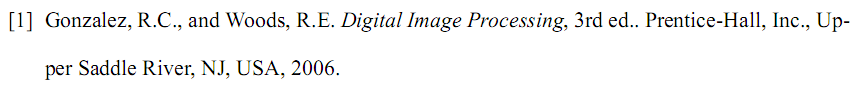
\includegraphics[width=\textwidth]{gonzalez.png}

این شیوهٔ تعریف مراجع بسیار ابتدایی است و اگر فرمت مراجع، ترتیب یا تعداد آنها را خواسته باشید تغییر دهید، به عنوان مثال ابتدا حرف اول نام نویسنده بیاید و سپس نام خانوادگی، باید همه کارها را به صورت دستی انجام دهید!
چون در یک \پ یا مقاله باید کنترل کاملی بر مراجع خود داشته باشید و به راحتی بتوانید قالب مراجع را عوض کنید، بنابراین می‌بایست از \lr{Bib\TeX} استفاده کنید که درپیوست  \ref{app:refMan} به  آن پرداخته خواهد شد.
		% پیوست اول: آشنایی مقدماتی با لاتک
%% !TeX root=../main.tex

\chapter{‌جدول، نمودار و الگوریتم در لاتک}
\label{app:latex:more}
%\thispagestyle{empty}

در این بخش نمونه مثالهایی از جدول، شکل، نمودار، الگوریتم و معادلات ریاضی را در لاتک خواهیم دید.
دقت کنید که در پایان‌نامه‌ها و مقالات، باید قاعدهٔ «ارجاع به جلو%
\LTRfootnote{Forward Referencing}»
رعایت شود؛ یعنی ابتدا در متن به شمارهٔ شکل، جدول یا معادله اشاره شود و بعد از آن (زیر آن) خود شکل، جدول یا معادله رسم شود. (توضیحات بیشتر در قسمت
\ref{sec:floatObjs}).

\section{جدول}
دستور اصلی برای رسم جدول در لاتک 
\verb|tabular|
می‌باشد که جدول
\eqref{tab:motionModels}
با استفاده از آن کشیده شده است؛ در
\verb|tabular|
عرض جدول برابر با مجموع عرض ستون‌ها و حداکثر مساوی عرض متن است.
\begin{table}[ht]
\caption{مدلهای تبدیل.}
\label{tab:motionModels}
\centering
\onehalfspacing
\begin{tabular}{|r|c|l|r|}
	\hline نام مدل & درجه آزادی & تبدیل مختصات & توضیح \\ 
	\hline انتقالی & ۲ & $\begin{aligned} x'=x+t_x \\ y'=y+t_y \end{aligned}$  &  انتقال دوبعدی\\ 
	\hline اقلیدسی & ۳ & $\begin{aligned} x'=x\cos\theta - y\sin\theta+t_x \\ y'=x\sin\theta+y\cos\theta+t_y \end{aligned}$  &  انتقالی+دوران \\ 
	\hline 
\end{tabular} 
\end{table}

برای اینکه عرض جدول قابل کنترل باشد، باید از دستورات
\verb|tabularx|،
\verb|tabulary| یا
\verb|tabu|
استفاده کرد که راهنمای آنها در اینترنت وجود دارد.
مثلاً جدول
\ref{tab:motionModelsCont}
با
\verb|tabularx|
رسم شده که عرض جدول در آن ثابت بوده و ستون‌های از نوع
\verb|X|
عرض خالی جدول را پر می‌کنند.
\begin{table}[ht]
	\caption{مدلهای تبدیل دیگر.}
	\label{tab:motionModelsCont}
	\centering
	\onehalfspacing
	\begin{tabularx}{\textwidth}{|r|c|l|X|}
		\hline نام مدل & درجه آزادی & تبدیل مختصات & توضیح \\ 
		\hline مشابهت & ۴ & $\begin{aligned} x'=sx\cos\theta - sy\sin\theta+t_x \\ y'=sx\sin\theta+sy\cos\theta+t_y  \end{aligned}$  & اقلیدسی+تغییرمقیاس \\ 		
		\hline آفین & ۶ & $\begin{aligned} x'=a_{11}x+a_{12}y+t_x \\ y'=a_{21}x+a_{22}y+t_y \end{aligned}$  & مشابهت+اریب‌شدگی \\
		\hline
	\end{tabularx}
\end{table}

\section{معادلات ریاضی و ماتریس‌ها}
تقریباً هر آنچه دانشجویان برای نوشتن فرمول‌های ریاضی لازم دارند، در کتاب 
\lr{mathmode}
آمده است. کافیست در خط فرمان، دستور زیر را وارد کنید:
\begin{latin}
	\texttt{texdoc mathmode}
\end{latin}
متن زیر شامل انواعی از اشیاء ریاضی است که با ملاحظه کدش می‌توانید با دستورات آن آشنا شوید.\\
شناخته‌شده‌ترین روش تخمین ماتریس هوموگرافی الگوریتم تبدیل خطی مستقیم (\lr{DLT\LTRfootnote{Direct Linear Transform}}) است.  فرض کنید چهار زوج نقطهٔ متناظر در دو تصویر در دست هستند،  $\mathbf{x}_i\leftrightarrow\mathbf{x}'_i$   و تبدیل با رابطهٔ
  $\mathbf{x}'_i = H\mathbf{x}_i$
  نشان داده می‌شود که در آن:
\[\mathbf{x}'_i=(x'_i,y'_i,w'_i)^\top  \]
و
\[ H=\left[
\begin{array}{ccc}
h_1 & h_2 & h_3 \\ 
h_4 & h_5 & h_6 \\ 
h_7 & h_8 & h_9
\end{array} 
\right]\]
رابطه زیر را برای الگوریتم  \eqref{alg:DLT} لازم داریم.
\begin{equation}
\label{eq:DLT_Ah}
\left[
\begin{array}{ccc}
	0^\top & -w'_i\mathbf{x}_i^\top & y'_i\mathbf{x}_i^\top \\ 
	w'_i\mathbf{x}_i & 0^\top & -x'_i\mathbf{x}_i^\top \\ 
	- y'_i\mathbf{x}_i^\top & x'_i\mathbf{x}_i^\top & 0^\top
\end{array} 
\right]
\left(
\begin{array}{c}
	\mathbf{h}^1 \\ 
	\mathbf{h}^2 \\ 
	\mathbf{h}^3
\end{array} 
\right)=0
\end{equation}

\section{الگوریتم}

\subsection{الگوریتم ساده با دستورهای فارسی}
با مفروضات فوق، الگوریتم \lr{DLT} به صورت نشان داده شده در الگوریتم \eqref{alg:DLT}  خواهد بود.
\begin{algorithm}[ht]
\onehalfspacing
\caption{الگوریتم \lr{DLT} برای تخمین ماتریس هوموگرافی.} \label{alg:DLT}
\begin{algorithmic}[1]
\REQUIRE $n\geq4$ زوج نقطهٔ متناظر در دو تصویر 
${\mathbf{x}_i\leftrightarrow\mathbf{x}'_i}$،\\
\ENSURE ماتریس هوموگرافی $H$ به نحوی‌که: 
$\mathbf{x}'_i = H \mathbf{x}_i$.
  \STATE برای هر زوج نقطهٔ متناظر
$\mathbf{x}_i\leftrightarrow\mathbf{x}'_i$ 
ماتریس $\mathbf{A}_i$ را با استفاده از رابطهٔ \ref{eq:DLT_Ah} محاسبه کنید.
  \STATE ماتریس‌های ۹ ستونی  $\mathbf{A}_i$ را در قالب یک ماتریس $\mathbf{A}$ ۹ ستونی ترکیب کنید. 
  \STATE تجزیهٔ مقادیر منفرد \lr{(SVD)}  ماتریس $\mathbf{A}$ را بدست آورید. بردار واحد متناظر با کمترین مقدار منفرد جواب $\mathbf{h}$ خواهد بود.
  \STATE  ماتریس هوموگرافی $H$ با تغییر شکل $\mathbf{h}$ حاصل خواهد شد.
\end{algorithmic}
\end{algorithm}

\subsection{الگوریتم پیچیده و تودرتو با دستورهای فارسی}
الگوریتم \ref{alg:simulation-random}، یک الگوریتم ترکیبی و تودرتو است که با کمک دستورهای بستهٔ \lr{algorithmic} نوشته شده است.

\begin{algorithm}[p]
    \onehalfspacing
    \caption{الگوریتم اجرای برنامهٔ شبیه‌سازی}
    \label{alg:simulation-random}
    \begin{algorithmic}[1]
        \REQUIRE زمان $t_{max}$ به عنوان زمان لازم برای انجام شبیه سازی،\\
        \REQUIRE  گراف شبکه برای شبیه سازی،
        \ENSURE جدول تغییرات گراف از لحظهٔ ۰ تا t.
        \FOR {تمام لحظات در بازهٔ ۰ تا $t_{max}$}
            \FOR {تمام پیوند‌ها}
                \STATE محاسبهٔ ضریب و نرخ انتقال پیوند
                \STATE محاسبهٔ کیفیت و نرخ یادگیری
            \ENDFOR
            \FOR {تمام گره‌ها}
                \STATE محاسبهٔ نرخ انتقال گره
                \STATE محاسبهٔ وضعیت جدید
            \ENDFOR
            \IF {تغییرات از مقدار $\delta$ کمتر است}
                \STATE شکستن حلقه
                \COMMENT{این شرط برای پایان قبل از رسیدن به محدودیت زمانی است، اگر تغییرات کمتر از $\delta$ باشد}
            \ELSIF {زمان اجرای برنامه بیش از حد طول کشیده \AND $t>100$}
                \STATE شکستن حلقه
            \ENDIF
        \ENDFOR
        \PRINT {زمان اجرای برنامه}
        \RETURN {ماتریس تغییرات زمانی}
    \end{algorithmic}
\end{algorithm}

\subsection{الگوریتم با دستورهای لاتین}
الگوریتم \ref{alg:RANSAC} یک الگوریتم با دستورهای لاتین است.

\begin{algorithm}[ht]
\onehalfspacing
\caption{الگوریتم \lr{RANSAC} برای تخمین ماتریس هوموگرافی.} \label{alg:RANSAC}
\begin{latin}
\begin{algorithmic}[1]
\REQUIRE $n\geq4$ putative correspondences, number of estimations, $N$, distance threshold $T_{dist}$.\\
\ENSURE Set of inliers and Homography matrix $H$.
\FOR{$k = 1$ to $N$}
  \STATE Randomly choose 4 correspondence,
  \STATE Check whether these points are colinear, if so, redo the above step
  \STATE Compute the homography $H_{curr}$ by DLT algorithm from the 4 points pairs,
  \STATE $\ldots$ % الگوریتم کامل نیست
  \ENDFOR
  \STATE Refinement: re-estimate H from all the inliers using the DLT algorithm.
\end{algorithmic}
\end{latin}
\end{algorithm}

\section{کد}
درج کد به زبان‌های مختلف به سادگی امکان‌پذیر است. برنامه
\ref{code:matlabEx}
یک قطعه کد
\lr{MATLAB}
را نشان می‌دهد.
\begin{figure}[ht]
	\begin{LTR}
        \singlespacing
		\lstinputlisting[language=MATLAB, caption={نمونه کد \lr{MATLAB}}, label={code:matlabEx}]{MatlabExample.m}
        % \doublespacing
	\end{LTR}
\end{figure}

\section{تصویر}
نمونهٔ یک تصویر را در فصل قبل دیدیم. دو تصویر شیر کنار هم را نیز در شکل
\ref{fig:twoLion}
مشاهده می‌کنید.
\begin{figure}[ht]
\centering 
\subfloat[شیر ۱]{ \label{fig:twolion:one}

\includegraphics[width=0.3\textwidth]{lion}}
%\hspace{2mm}
\subfloat[شیر ۲]{ \label{fig:twolion:two}

\includegraphics[width=0.3\textwidth]{lion}}%
\caption{دو شیر}
\label{fig:twoLion} %% label for entire figure
\end{figure}

\section{نمودار}
لاتک بسته‌هایی با قابلیت‌های زیاد برای رسم انواع مختلف نمودارها دارد. مانند بسته‌های \lr{Tikz} و  \lr{PSTricks}. توضیح اینها فراتر از این پیوست کوچک است.%
\footnote{
مثال‌هایی از بکارگیری بسته
\lr{Tikz}
را می‌توانید در
\url{http://www.texample.net/tikz/examples/}
ببینید. توصیه می‌شود دانشجویانی که قصد درج اشکالی مانند گراف را در سند خود دارند، مثالهایی از سایت مذکور را ملاحظه فرمایند.
}
یک نمودار رسم شده با بستهٔ 
\lr{TikZ}
 در شکل 
\ref{fig:parabola}
نشان داده شده است.
\begin{figure}[t]
\centering
\begin{tikzpicture}[scale=2.5]
  \shade[top color=blue,bottom color=gray!50] 
      (0,0) parabola (1.5,2.25) |- (0,0);
  \draw (1.05cm,2pt) node[above] 
      {$\displaystyle\int_0^{3/2} \!\!x^2\mathrm{d}x$};

  \draw[style=help lines] (0,0) grid (3.9,3.9)
       [step=0.25cm]      (1,2) grid +(1,1);

  \draw[->] (-0.2,0) -- (4,0) node[right] {$x$};
  \draw[->] (0,-0.2) -- (0,4) node[above] {$f(x)$};

  \foreach \x/\xtext in {1/1, 1.5/1\frac{1}{2}, 2/2, 3/3}
    \draw[shift={(\x,0)}] (0pt,2pt) -- (0pt,-2pt) node[below] {$\xtext$};

  \foreach \y/\ytext in {1/1, 2/2, 2.25/2\frac{1}{4}, 3/3}
    \draw[shift={(0,\y)}] (2pt,0pt) -- (-2pt,0pt) node[left] {$\ytext$};

  \draw (-.5,.25) parabola bend (0,0) (2,4) node[below right] {$x^2$};
\end{tikzpicture}
\caption{یک نمودار زیبا با ارقام فارسی و قابلیت بزرگ‌نمایی بسیار، بدون از دست دادن کیفیت.}
\label{fig:parabola}
\end{figure}

\section{نحوه قرارگیری اشیای شناور}
\label{sec:floatObjs}
شکل‌ها، جداول و الگوریتم‌ها در لاتک اشیای شناور محسوب می‌شوند؛ یعنی خود لاتک تصمیم می‌گیرد آنها را در کجای صفحه ترسیم کند تا زیباتر باشد. اما می‌توان به لاتک توصیه کرد که آن را در قسمت خاصی از صفحه رسم کند. برای اینکه قاعدهٔ «ارجاع به جلو» رعایت شود باید فقط از پرچم
\verb|[ht]|
استفاده کرد، که می‌گوید اگر جا شد شکل را دقیقاً در همین مکان و در غیراینصورت در بالای صفحه بعد رسم کن.
بنابراین دستورات درج تصویر، جدول و الگوریتم به صورت زیر باید باشند:

\begin{latin}
\begin{verbatim}
	\begin{figure/table/algorithm}[ht]
		...
	\end{figure/table/algorithm}
\end{verbatim}
\end{latin}
		% پیوست دوم: جدول، نمودار و الگوریتم در لاتک
%% !TeX root=../main.tex
\chapter{مراجع، واژه‌نامه و حاشیه‌نویسی}
\label{app:refMan}
%\thispagestyle{empty}

\section{مراجع و نقل‌قول‌ها}
\label{sec:refUsage}
منابعِ پایان‌نامه، پایه و اساس تحقیق شما به حساب می‌آیند و ضرورت انجام مطالعه و روش‌های به کار رفته در بسیاری از قسمت‌های آن، به کمک منابع صورت می‌گیرد. در استفاده از مراجع علمی در پایان‌نامه، باید سعی کنید بیشتر از
\textbf{منابع چاپ‌شده و مهم}
استفاده کنید و
\emph{ارجاع به داده‌های چاپ نشده، خلاصه‌ها و پایان‌نامه‌ها، سبب به‌هم‌خوردگی و کاهش اعتبار قسمت ارجاع منابع می‌شود.}
استفاده از منابع و نقل قول‌هایی به تحقیق شما ارزش می‌دهند که
\textbf{در راستای هدف تحقیق بوده و به آن اعتبار ببخشند.}
برخی از دانش‌جویان تصوّر می‌کنند که کثرت نقل‌قول‌ها و ارجاعات زیاد، مهم‌ترین معیار علمی شدن پایان‌نامه است؛ حال آنکه استناد به تعداد کثیری از منابع بدون مطالعه دقیق آنها و استفادهٔ مستقیم در پایان‌نامه، می‌تواند نشان‌دهندهٔ عدم احساس امنیت نویسنده باشد!

دو روش برای استفاده از نتایج، جملات، داده‌ها و روش‌های دیگران وجود دارد. یکی نقل‌قول مستقیم و دقیق است و دیگری استفاده غیرمستقیم در متن مقاله، که در ادامه به قواعد این دو نوع نقل‌قول و ارجاع‌دهی اشاره می‌کنیم:
\begin{description}
	\item[نقل‌قول مستقیم:]
	نقل‌قول مستقیم باید دقیق و بدون هیچ تغییری در جملات باشد. بهتر است این‌گونه نقل‌قول‌ها تا حد امکان کوتاه باشد. جملات کوتاه داخل گیومه قرار می‌گیرند و باید به منبع دقیق آن، طبق روش ارجاع‌دهی به منابع، اشاره شود. به عنوان مثال در
	\cite{persianbib87userguide}
	آمده است که:
	\begin{quote}
		«با استفاده از فیلد
		\lr{AUTHORFA}
		می‌توان معادل فارسی نام نویسندگان مقالات لاتین را در متن داشت. معمولاً در اسناد فارسی خواسته می‌شود که پس از ذکر معادل فارسی نام نویسنده، نام لاتین نویسنده(ها) به عنوان پاورقی درج شود
		\citep{persianbib87userguide}.»
	\end{quote}
	\item[نقل‌قول غیرمستقیم:]
	نقل‌قول غیرمستقیم به معنی استفاده از ایده‌ها، نتایج، روش‌ها و داده‌های دیگران در درون متنِ پایان‌نامه، ولی به سبک خودتان و متناسب و هماهنگ با روند پایان‌نامهٔ شماست. در این حالت نیز باید متناسب با شیوهٔ ارجاع‌دهی به آن استناد شود.
\end{description}

با توجه به وجود سبک‌های مختلف ارجاع‌دهی، باید
\textbf{روش قابل قبول و یکسانی}
در طول پایان‌نامه برای اشاره به مراجع در متن و همچنین تهیه فهرست مراجع در انتهای پایان‌نامه بکار رود. مثلاً برای پایان‌نامه‌های مهندسی می‌توان از سبک ارجاع‌دهی
\lr{IEEE}%
\LTRfootnote{\url{http://www.ieee.org/documents/ieeecitationref.pdf}}
یا
\lr{acm}
استفاده کرد. طبیعتاً باید تناظر یک‌به‌یک بین فهرست مراجع در انتهای گزارش و مراجع مورد استفاده در متن باشد%
\footnote{البته گاهی ممکن است محقق مرجعی را مورد مطالعه قرار داده لیکن در متن به آن اشاره نکرده باشد؛ برخی معتقدند در این موارد نیز آوردن آن در فهرست مراجع، اشکالی ندارد، به این شرط که از عنوان «فهرست منابع» به جای «فهرست مراجع» استفاده شود.}.

برای سهولت مدیریت مراجعِ \پ%
، اکیداً توصیه می‌شود از یک ابزار «مدیریت منابع» (با خروجی
\texorpdfstring{\lr{Bib\TeX}}{Bib\TeX}%
) همچون
\lr{Mendeley}،
\lr{Zotero},
\lr{EndNote}
یا
\lr{Citavi}
استفاده کنید.

\subsection{ مدیریت مراجع با  \texorpdfstring{\lr{Bib\TeX}}{Bib\TeX}}
در بخش \ref{Sec:Ref} اشاره شد که با دستور 
 \lr{\textbackslash bibitem}
  می‌توان یک مرجع را تعریف نمود و با فرمان
 \lr{\textbackslash cite}
  به آن ارجاع داد. این روش برای تعداد مراجع زیاد و تغییرات آنها مناسب نیست. برای مدیریت منابع زیاد، سه بستهٔ
\lr{BibTeX} (پیش‌فرض),
\lr{natbib}
(ارجاع‌دهی در متن به صورت نویسنده-سال)
و \lr{BibLaTeX} (جدید و منعطف‌پذیر)
وجود دارند. در ادامه توضیحاتی در مورد مدیریت منابع با \lr{BibTeX} و \lr{natbib} در زی‌پرشین خواهیم آورد که همراه با توزیع‌های معروف تِک عرضه می‌شوند
\footnote{روش \lr{BibLaTeX} هنوز برای متون فارسی به درستی ترجمه نشده است.}.

یکی از روش‌های قدرتمند و انعطاف‌پذیر برای نوشتن مراجعِ مقالات و مدیریت مراجع در لاتک، استفاده از  \lr{BibTeX} است.
 روش کار با بیب‌تک به این صورت است که مجموعهٔ همهٔ مراجعی را که در \پ استفاده کرده یا خواهیم کرد، 
در پروندهٔ جداگانه‌ای با پسوند
\lr{bib}
نوشته و به آن فایل در سند خودمان به صورت مناسب لینک می‌دهیم.
 کنفرانس‌ها یا مجله‌های گوناگون برای نوشتن مراجع، قالب‌ها یا قراردادهای متفاوتی دارند که به آنها استیل‌های مراجع گفته می‌شود.
 در این حالت به کمک ‌استیل‌های بیب‌تک خواهید توانست تنها با تغییر یک پارامتر در پروندهٔ ورودی خود، مراجع را مطابق قالب موردنظر تنظیم کنید. 
 بیشتر مجلات و کنفرانس‌های معتبر یک فایل سبک
 (\lr{BibTeX Style})
با پسوند \lr{bst} در وب‌گاه خود می‌گذارند که برای همین منظور طراحی شده است.

به جز نوشتن مقالات، این سبک‌ها کمک بسیار خوبی برای تهیهٔ مستندات علمی همچون پایان‌نامه‌هاست که فرد می‌تواند هر قسمت از کارش را که نوشت مراجع مربوطه را به بانک مراجع خود اضافه نماید. با داشتن چنین بانکی از مراجع، وی خواهد توانست به راحتی یک یا چند ارجاع به مراجع و یا یک یا چند بخش را حذف یا اضافه ‌نماید؛ 
مراجع به صورت خودکار مرتب شده و
\textbf{فقط مراجع ارجاع داده شده در قسمت کتاب‌نامه خواهندآمد.}
قالب مراجع به صورت یکدست مطابق سبک داده شده بوده و نیازی نیست که کاربر درگیر قالب‌دهی به مراجع باشد. 

\subsection{سبک‌های مورد تأیید دانشگاه تهران}
طبق «دستورالعمل نگارش و تدوین پایان‌نامه» دانشگاه تهران در
\cite{UTThesisGuide}،
ارجاع در متن می‌تواند مطابق با هر یک از دو الگوی هاروارد یا ونکوور باشد:
\singlespacing
\begin{description}
	\item[سیستم نویسنده-سال (هاروارد):]
	ذکر نام نویسنده و سال نشر در متن. در این الگو مراجع بر اساس حروف الفبا تنظیم می‌گردند.
	\item[سیستم شماره‌دار (ونکوور):]
	ارجاع به مراجع به کمک شماره در متن. در این الگو شماره هر مرجع به ترتیب ظاهر شدن آن در متن در داخل کروشه قرار می‌گیرد. فهرست مراجع نیز بر اساس شماره مرجع (نه حروف الفبا) تنظیم می‌گردد.
\end{description}
\doublespacing

در مدیریت منابع با
\lr{\textbf{BibTeX}}،
ارجاع‌ها در متن تنها به شکل
\textbf{شماره‌دار (ونکوور)}
امکان‌پذیر است، گرچه فهرست مراجع می‌تواند با روش‌های مختلف مرتب شود. اگر بخواهیم ارجاع‌ها در متن به صورت
\textbf{نویسنده-سال (هاروارد)}
باشد باید از بستهٔ
\lr{\textbf{natbib}}\LTRfootnote{Natural Sciences Citations \& References}
و استیل‌های مختلف آن استفاده کنیم.

هنگام استفاده از روش نویسنده-سال نوع پرانتزگذاری‌ها در وسط و انتهای جمله با هم فرق خواهد داشت. به مثال زیر مطابق با دستورالعمل
\cite{UTThesisGuide}
توجه کنید:

\textit{
ابتدا
\cite{Khalighi87xepersian}
بستهٔ زی‌پرشین را برای حروف‌چینی فارسی اختراع کرد. بعدها سبک‌های ارجاع‌دهی فارسی و قالب‌های پایان‌نامه نیز مبتنی بر آن ساخته شد
\citep{persianbib87userguide}.
ارجاع‌دهی به مراجع لاتین نیز در زی‌پرشین امکان‌پذیر است. مثلاً
\citelatin{Gonzalez02book}
یک کتاب انگلیسی است و به راحتی به مقالات انگلیسی نیز می‌توان ارجاع داد
\citeplatin{kim2016integrated}.}

در این مثال، ۴ ارجاع در وسط و انتهای جمله به مراجع فارسی و انگلیسی آمده است. وقتی از سیستم نویسنده-سال استفاده می‌کنید، بهتر است ارجاع‌های آخر جمله کلاً داخل پرانتر بیاید؛ بدین منظور باید به جای
\verb|\cite|
از
\verb|\citep|
استفاده کنید. اما در سیستم شماره‌دار چون تمام ارجاع‌ها داخل کروشه می‌آیند این امر اهمیت ندارد.\\
نمی‌توانید در متن فارسی، اسم لاتین محقق خارجی را بیاورید و برای جلوگیری از ایجاد ابهام، صرف‌نظر از نام لاتین هم مجاز نیست! توصیه می‌شود که نام محقق خارجی در متن با حروف فارسی و در پاورقی اسم تمام نویسندگان به صورت انگلیسی آورده شود. نحوهٔ رعایت این نکته را می‌توانید در کد مثال بالا ببینید.

گرچه در تمپلت ورد
\cite{UTThesisGuide}،
به صراحت ذکر شده که بهتر است برای پایان‌نامه‌های مهندسی از سبک 
\lr{IEEE}
استفاده شود (که از سیستم ونکوور تبعیت می‌کند)، اما ترتیب فهرست مراجع در
\lr{IEEE}
بر اساس ترتیب ارجاع در متن بوده و
\emph{مراجع انگلیسی و فارسی از هم تفکیک نمی‌شوند}
که متضاد با دستورالعمل
\cite{UTThesisGuide}
و نیز متضاد عرف اکثر پایان‌نامه‌های فارسی است.
بنابراین دقیقاً نمی‌توان سبک خاصی را برای مراجع پایان‌نامه‌های دانشگاه تهران اجبار کرد. مهم این است که
\textbf{سبک ارجاع‌دهی در تمام طول یک کتابچه}
(مثلاً پایان‌نامه، مقالات یک مجله یا کل یک کتاب) یکسان باشد. بهتر است
\textbf{بسته به حوزه پایان‌نامه}،
در این مورد با استاد راهنمای خود مشورت کنید.

\subsection{سبک‌های فارسی قابل استفاده در زی‌پرشین}
تعدادی از سبک‌های فارسی بسته
\lr{Persian-bib}%
\footnote{ برای اطلاع بیشتر به راهنمای بستهٔ
\lr{Persian-bib}
مراجعه فرمایید.}
که برای  زی‌پرشین آماده شده‌اند، عبارتند از:

\singlespacing
\begin{itemize}
\item \emph{سبک‌های شماره‌دار}:
	\begin{description}
	\item [unsrt-fa.bst] این سبک متناظر با \lr{unsrt.bst} می‌باشد. مراجع به ترتیب ارجاع در متن ظاهر می‌شوند.
	\item [plain-fa.bst] این سبک متناظر با \lr{plain.bst} می‌باشد. مراجع بر اساس نام‌خانوادگی نویسندگان، به ترتیب صعودی مرتب می‌شوند.
	 همچنین ابتدا مراجع فارسی و سپس مراجع انگلیسی خواهند آمد.
	\item [acm-fa.bst] این سبک متناظر با \lr{acm.bst} می‌باشد. شبیه \lr{plain-fa.bst} است.  قالب مراجع کمی متفاوت است. اسامی نویسندگان انگلیسی با حروف بزرگ انگلیسی نمایش داده می‌شوند. (مراجع مرتب می‌شوند)
	\item [ieeetr-fa.bst] این سبک متناظر با \lr{ieeetr.bst} می‌باشد. (مراجع مرتب نمی‌شوند)
	\end{description}
	
\item \emph{سبک‌های نویسنده-سال}:
	\begin{description}
	\item [plainnat-fa.bst] این سبک متناظر با \lr{plainnat.bst} می‌باشد. نیاز به بستهٔ \lr{natbib} دارد. (مراجع مرتب می‌شوند)
	\item [chicago-fa.bst] این سبک متناظر با \lr{chicago.bst} می‌باشد. نیاز به بستهٔ \lr{natbib} دارد. (مراجع مرتب می‌شوند)
	\item [asa-fa.bst] این سبک متناظر با \lr{asa.bst} می‌باشد. نیاز به بستهٔ \lr{natbib} دارد. (مراجع مرتب می‌شوند)
	\end{description}
\end{itemize}
\doublespacing

با استفاده از استیل‌های فوق می‌توانید به انواع مختلفی از مراجع فارسی و لاتین ارجاع دهید.
به عنوان مثال‌هایی از
\textbf{مراجع انگلیسی}،
مرجع
\cite{Baker02limits}\footnote{چون فیلد \lr{authorfa} برای این مرجع تعریف نشده در سبک نویسنده-سال با حروف لاتین به آن در متن ارجاع می‌شود که غلط است.}
مقالهٔ یک ژورنال، مرجع
\cite{Amintoosi09video}
مقالهٔ یک کنفرانس، مرجع
\citelatin{Gonzalez02book}
یک کتاب، مرجع
\cite{Khalighi07MscThesis}
پایان‌نامهٔ کارشناسی ارشد و مرجع
\citelatin{Borman04thesis}
یک رسالهٔ دکتری می‌باشد.\\
همچنین در میان
\textbf{مراجع فارسی},
مرجع
\cite{Vahedi87}
مقالهٔ یک مجله، مرجع
\cite{Amintoosi87afzayesh}
مقالهٔ یک کنفرانس، مرجع
\cite{Pedram80osool}
یک کتاب ترجمه‌شده با ذکر مترجمان و ویراستاران، مرجع
\cite{Pourmousa88mscThesis}
پایان‌نامهٔ کارشناسی ارشد%
\footnote{همان‌طور که در بخش
\ref{sec:refUsage}
اشاره شد، بهتر است زیاد از پایان‌نامه‌ها در مراجع استفاده نکنید.}،
مرجع
\cite{Omidali82phdThesis}
یک رسالهٔ دکتری و مراجع
\cite{persianbib87userguide, Khalighi87xepersian}
نمونه‌های متفرقه هستند.

\subsection{ساختار فایل مراجع}
برای استفاده از بیب‌تک باید مراجع خود را در یک فایل با پسوند \lr{bib} ذخیره نمایید. یک فایل \lr{bib} در واقع یک پایگاه داده از مراجع%
\LTRfootnote{Bibliography Database}
شماست که هر مرجع در آن به عنوان یک رکورد از این پایگاه داده
با قالبی خاص ذخیره می‌شود. به هر رکورد یک مدخل%
\LTRfootnote{Entry}
گفته می‌شود. یک نمونه مدخل برای معرفی کتاب \lr{Digital Image Processing} در ادامه آمده است:

\singlespacing
\begin{LTR}
\begin{verbatim}
@BOOK{Gonzalez02image,
  AUTHOR     = {Gonzalez,, Rafael C. and Woods,, Richard E.},
  TITLE      = {Digital Image Processing},
  PUBLISHER  = {Prentice-Hall, Inc.},
  YEAR       = {2006},
  ISBN       = {013168728X},
  EDITION    = {3rd},
  ADDRESS    = {Upper Saddle River, NJ, USA}
}
\end{verbatim}
\end{LTR}
\doublespacing

در مثال فوق، \lr{@BOOK} مشخصهٔ شروع یک مدخل مربوط به یک کتاب و \lr{Gonzalez02book} برچسبی است که به این مرجع منتسب شده است.
 این برچسب بایستی یکتا باشد. برای آنکه بتوان
\textbf{برچسب مراجع}
 را به راحتی به خاطر سپرد و حتی‌الامکان برچسب‌ها متفاوت با هم باشند، معمولاً از قوانین خاصی به این منظور استفاده می‌شود. یک قانون می‌تواند
\textbf{فامیل نویسنده اول + دورقم سال نشر + اولین کلمهٔ عنوان اثر}
باشد. به
\lr{AUTHOR}، \lr{TITLE}، $\dots$ و \lr{ADDRESS}
فیلدهای این مدخل گفته می‌شود، که هر یک با مقادیر مربوط به مرجع پر شده‌اند. ترتیب فیلدها مهم نیست. 

انواع متنوعی از مدخل‌ها برای اقسام مختلف مراجع همچون کتاب، مقالهٔ کنفرانس و مقالهٔ ژورنال وجود دارد که برخی فیلدهای آنها با هم متفاوت است. 
نام فیلدها بیانگر نوع اطلاعات آن می‌باشد. مثالهای ذکر شده در فایل \lr{MyReferences.bib} کمک خوبی برای شما خواهد بود. 
%این فایل یک فایل متنی بوده و با ویرایشگرهای معمول همچون \lr{Notepad++} قابل ویرایش می‌باشد. برنامه‌هایی همچون 
%\lr{TeXMaker}
% امکاناتی برای نوشتن این مدخل‌ها دارند و به صورت خودکار فیلدهای مربوطه را در فایل \lr{bib}  شما قرار می‌دهند.  
با استفاده از سبک‌های فارسی آماده شده، محتویات هر فیلد می‌تواند به فارسی نوشته شود؛ ترتیب مراجع و نحوهٔ چینش فیلدهای هر مرجع را سبک مورد استفاده  مشخص خواهد کرد.

\textbf{در فایل 
\lr{MyReferences.bib}
 که همراه با این \پ هست، مثال‌های مختلفی از مراجع آمده‌اند که برای درج مراجع خود، تنها کافیست مراجع‌تان را جایگزین موارد مندرج در آن نمایید.
}

برای بسیاری از مقالات لاتین حتی لازم نیست که مدخل مربوط به آنرا خودتان بنویسید. با جستجوی 
\textbf{نام مقاله + کلمه
\lr{bibtex}}
در اینترنت سایت‌های بسیاری همچون
\lr{ACM} و \lr{ScienceDirect}
را خواهید یافت که مدخل
\lr{bibtex}
مربوط به مقاله شما را دارند و کافیست آنرا به انتهای فایل
\lr{MyReferences.bib}
اضافه کنید.

\subsection{نحوه اجرای \texorpdfstring{\lr{Bib\TeX}}{Bib\TeX}}
پس از قرار دادن مراجع خود، برای ساخت فایل خروجی می‌توانید دستور زیر را (در ترمینال یا از طریق \lr{Texmaker}) اجرا کنید:%
\footnote{فایل \lr{latexmkrc} باید در کنار \lr{main.tex} وجود داشته باشد.}

\singlespacing
\begin{LTR}
	\begin{verbatim}
		latexmk -bibtex -pdf main.tex
	\end{verbatim}
\end{LTR}
\doublespacing
ابزار \lr{latexmk} مراحل مختلف ساخت خروجی لاتک را به طور خودکار و بهینه انجام می‌دهد و هر بار فقط مراحلی را که لازم باشد تکرار می‌کند.
روش دستی‌تر این است که یک بار \lr{XeLaTeX} را روی سند خود اجرا نمایید، سپس \lr{bibtex} و پس از آن هم ۲ بار \lr{XeLaTeX} را. در \lr{TeXMaker} کلید \lr{F11} و در \lr{TeXWorks} هم گزینهٔ \lr{BibTeX} از منوی \lr{Typeset}، \lr{BibTeX} را روی سند شما اجرا می‌کنند.

\section{واژه‌نامه‌ها و فهرست اختصارات}
\gls{Gloss}
یا فرهنگ لغات، مجموعه‌ای از اصطلاحات و تعاریف خاص و فنی است که معمولاً در انتهای یک کتاب می‌آید. چون پایان‌نامه خود یک متن تخصصی بلند محسوب می‌شود، استفاده از فرهنگ لغات در انتهای آن به شدت توصیه می‌شود، خصوصاً که احتمال استفاده از لغات تخصصی لاتین در آن بالاست.
واژه‌نامه‌هایی که در انتهای کتاب‌های انگلیسی می‌آیند معمولاً تک‌زبانه هستند و معنی یک اصطلاح تخصصی در آنها، عمدتاً به صورت یک
\gls{Description}
طولانی آورده می‌شود. اما چون در متون فارسی، آوردن لغات انگلیسی مجاز نیست و باید معادل فارسی آنها وارد شود، جهت رفع ابهام معمولاً واژه‌نامهٔ فارسی به انگلیسی (و برعکس) در انتهای کتاب درج شده و  
\glspl{Description}
در صورت نیاز در متن آورده می‌شوند.

فهرست
\glspl{Acronym}
شامل نمادهای کوتاهی است که اغلب از حروف ابتدایی کلمات یک عبارت طولانی ساخته شده‌اند. با اینکه
\glspl{Acronym}
با حروف (بزرگ) لاتین نوشته می‌شوند، اما چون کوتاهند استفاده از آنها در میان متن فارسی مجاز است. با این حال برای رفع ابهام، عرف است که فهرستی از آنها شامل معنی هر نماد، در کنار دیگر فهرست‌ها در ابتدای متن درج شود.

در این قالب پایان‌نامه، برای ساخت و مدیریت واژه‌نامه و فهرست اختصارات از بستهٔ پیشرفتهٔ
\lr{glossaries}
با موتور واژه‌نامه‌سازی
\lr{xindy}
استفاده می‌شود. تنظیمات بهینهٔ این بسته در فایل
\lr{glossaries-settings.tex}
عبارتند از:
\begin{itemize}
	\item
قبل از درج واژه‌ها در متن، باید مدخل آنها با دستور زیر (ترجیحاً در فایل جدای \lr{words.tex}) تعریف شود:
	\begin{LTR}
	\verb|\newword{Label}{Word}|\{واژه\}\{واژه‌ها\}
	\end{LTR}
	
	\item
قبل از وارد کردن علائم اختصاری در متن، باید مدخل آنها نیز (ترجیحاً در فایل \lr{acronyms.tex}) به صورت زیر تعریف شود:
	\begin{LTR}
	\verb|\newacronym{Label}{Acr}|\{معنی‌اختصار\}
	\end{LTR}

	\item
جهت درج یک علامت اختصاری یا معادل یک واژه تخصصی، کافی است از دستور
	\verb|gls{Label}|
در متن استفاده کنید. دستور
	\verb|glspl{Label}|
نیز برای آوردن معادل یک لغت در حالت جمع ساخته شده است.
	
	\item
هنگام اولین استفاده از یک معادل فارسی یا اختصار در متن، معادل انگلیسی یا معنی آن در پاورقی آورده می‌شود. در صورتی که هر یک از این پیش‌فرض‌ها را دوست ندارید با ویرایش فایل
	\lr{glossaries-settings.tex}
می‌توانید آن را تغییر دهید.

	\item
در انتهای پایان‌نامه با دستور
\verb|\printglossary|
فهرست کلمات استفاده‌شده به ترتیب الفبای فارسی (واژه‌نامه فارسی به انگلیسی) و الفبای انگلیسی (واژه‌نامه انگلیسی به فارسی) درج می‌شود.
\end{itemize}

به عنوان مثال، با مشاهدهٔ کد این نوشته، نحوهٔ درج معادل فارسی
\gls{RandomVariable}
را در متن مشاهده می‌کنید.
در نمایش واژهٔ
\gls{RandomVariable}
برای بار دوم، معادل لاتین در پاورقی نمی‌آید.
در مورد درج علائم اختصاری، مثلاً می‌توان به رابطهٔ
\gls{F}
اشاره کرد.

\section{حاشیه‌نویسی در نسخه پیش‌نویس}
اصلاح و بازبینی چندین و چندبارهٔ یک پایان‌نامه یا مقاله، از معمول‌ترین امور در نگارش آن می‌باشد. فرض کنید دانشجو پایان‌نامه یا مقالهٔ خود را (کامل یا ناقص) نوشته و می‌خواهد نظر استاد راهنما، اعضای آزمایشگاه یا دیگر متخصصین را در مورد آن جویا شود. به جز مشاورهٔ حضوری، تلفنی یا از طریق ایمیل، برای اظهارنظر دقیق بر نوشته، می‌توان از ابزارهای حاشیه‌نویسی در فایل
\lr{PDF}
یا \lr{tex}
نیز استفاده کرد.

یک راهکار مناسب برای حاشیه‌نویسی در فایل \lr{tex}، استفاده از بسته 
\lr{todonotes}
می‌باشد که آقای خلیقی به تازگی امکان استفاده از آن را برای فارسی‌زبانان نیز فراهم آورده‌اند.
بدین منظور، هر جایی که خواستید نکته یا نکاتی را در حاشیه متن یادداشت کنید، کافی است دستور زیر را وارد نمایید:
\begin{latin}
\verb|\todo{NOTE}|
\end{latin}
مثلاً استاد راهنما می‌تواند از دانشجو بخواهد که در بخشی توضیح بیشتری دهد.
\todo{
توضیح بیشتری لازم است.
}
استاد راهنما یا داور حتی می‌تواند محل پیشنهادی برای درج یک تصویر را نیز به راحتی برای دانشجو مشخص کند.
\missingfigure[figwidth=\textwidth,figcolor=white]{یک تصویر از خروجی الگوریتم 
\ref{alg:RANSAC}
را در اینجا قرار دهید.}
یکی دیگر از امکانات این بسته آن است که می‌توان فهرست نکات را در ابتدای سند داشت. بسته 
\lr{todonotes}
امکانات بسیاری دارد
\todo[fancyline,color=green!30]{مرجع این مطلب؟}
که در راهنمای آن معرفی شده است و با اجرای دستور زیر در خط فرمان می‌توانید آنها را مشاهده کنید:
\begin{latin}	
	\texttt{texdoc todonotes}
\end{latin}	
دقت کنید که توضیحات حاشیه‌ای و فهرست کارهای باقیمانده (نکات)،
\textbf{فقط در نسخه
\gls{Draft}}
قابل دیدن هستند و در نسخه نهایی، نمایش داده نخواهند شد.
برای استفاده از حالت
\gls{Draft}
باید گزینه 
\lr{draft}
به دستور 
\verb|\documentclass|
در ابتدای فایل 
\lr{main.tex}
اضافه شود.
هنگامی‌که سند شما در حالت 
\gls{Draft}
باشد:

\singlespacing
\begin{enumerate}
\item 
هیچ یک از صفحات آغازین پایان‌نامه، تا فهرست مطالب نمایش داده نمی‌شود (به جز صفحه اول).
\item
روی صفحه اول عبارت «پیش‌نویس» به صورت درشت و کم‌رنگ نمایش داده می‌شود.
\item
فهرست نکات درج شده توسط
\lr{todo}،
پس از فهرست اصلی و با عنوان «فهرست کارهای باقیمانده» نمایش داده می‌شود.
\item
شماره صفحاتی که به هر مرجع ارجاع داده شده است در بخش مراجع نمایش داده می‌شود
\footnote{اعمال گزینهٔ
\lr{pagebackref}
برای بستهٔ
\lr{hyperref}.
}.
\end{enumerate}
\doublespacing
هر یک از موارد بالا تا زمانی که نسخه نهایی \پ نیاز نباشد بسیار مورد توجه و مفید واقع می‌شوند.
   	% پیوست سوم: مراجع، واژه‌نامه و حاشیه‌نویسی

% برگرداندن شماره‌بندی صفحات فصول
% \let\chapter\Chapter
\pagenumbering{tartibi} % اول، دوم، ...
%\baselineskip=.75cm

% چاپ واژه‌نامه‌ها و نمایه 
\onehalfspacing
\cleardoublepage
\printglossary
\cleardoublepage
\printindex

\begin{latin}
\baselineskip=.6cm
\latinabstract
\latinTitlePage
\end{latin}
\label{LastPage}

\end{document}